\documentclass[]{article}
\usepackage{lmodern}
\usepackage{amssymb,amsmath}
\usepackage{ifxetex,ifluatex}
\usepackage{fixltx2e} % provides \textsubscript
\ifnum 0\ifxetex 1\fi\ifluatex 1\fi=0 % if pdftex
  \usepackage[T1]{fontenc}
  \usepackage[utf8]{inputenc}
\else % if luatex or xelatex
  \ifxetex
    \usepackage{mathspec}
  \else
    \usepackage{fontspec}
  \fi
  \defaultfontfeatures{Ligatures=TeX,Scale=MatchLowercase}
\fi
% use upquote if available, for straight quotes in verbatim environments
\IfFileExists{upquote.sty}{\usepackage{upquote}}{}
% use microtype if available
\IfFileExists{microtype.sty}{%
\usepackage{microtype}
\UseMicrotypeSet[protrusion]{basicmath} % disable protrusion for tt fonts
}{}
\usepackage[margin=1in]{geometry}
\usepackage{hyperref}
\hypersetup{unicode=true,
            pdftitle={Building patient-level predictive models},
            pdfauthor={Jenna Reps, Martijn J. Schuemie, Patrick B. Ryan, Peter R. Rijnbeek},
            pdfborder={0 0 0},
            breaklinks=true}
\urlstyle{same}  % don't use monospace font for urls
\usepackage{color}
\usepackage{fancyvrb}
\newcommand{\VerbBar}{|}
\newcommand{\VERB}{\Verb[commandchars=\\\{\}]}
\DefineVerbatimEnvironment{Highlighting}{Verbatim}{commandchars=\\\{\}}
% Add ',fontsize=\small' for more characters per line
\usepackage{framed}
\definecolor{shadecolor}{RGB}{248,248,248}
\newenvironment{Shaded}{\begin{snugshade}}{\end{snugshade}}
\newcommand{\KeywordTok}[1]{\textcolor[rgb]{0.13,0.29,0.53}{\textbf{#1}}}
\newcommand{\DataTypeTok}[1]{\textcolor[rgb]{0.13,0.29,0.53}{#1}}
\newcommand{\DecValTok}[1]{\textcolor[rgb]{0.00,0.00,0.81}{#1}}
\newcommand{\BaseNTok}[1]{\textcolor[rgb]{0.00,0.00,0.81}{#1}}
\newcommand{\FloatTok}[1]{\textcolor[rgb]{0.00,0.00,0.81}{#1}}
\newcommand{\ConstantTok}[1]{\textcolor[rgb]{0.00,0.00,0.00}{#1}}
\newcommand{\CharTok}[1]{\textcolor[rgb]{0.31,0.60,0.02}{#1}}
\newcommand{\SpecialCharTok}[1]{\textcolor[rgb]{0.00,0.00,0.00}{#1}}
\newcommand{\StringTok}[1]{\textcolor[rgb]{0.31,0.60,0.02}{#1}}
\newcommand{\VerbatimStringTok}[1]{\textcolor[rgb]{0.31,0.60,0.02}{#1}}
\newcommand{\SpecialStringTok}[1]{\textcolor[rgb]{0.31,0.60,0.02}{#1}}
\newcommand{\ImportTok}[1]{#1}
\newcommand{\CommentTok}[1]{\textcolor[rgb]{0.56,0.35,0.01}{\textit{#1}}}
\newcommand{\DocumentationTok}[1]{\textcolor[rgb]{0.56,0.35,0.01}{\textbf{\textit{#1}}}}
\newcommand{\AnnotationTok}[1]{\textcolor[rgb]{0.56,0.35,0.01}{\textbf{\textit{#1}}}}
\newcommand{\CommentVarTok}[1]{\textcolor[rgb]{0.56,0.35,0.01}{\textbf{\textit{#1}}}}
\newcommand{\OtherTok}[1]{\textcolor[rgb]{0.56,0.35,0.01}{#1}}
\newcommand{\FunctionTok}[1]{\textcolor[rgb]{0.00,0.00,0.00}{#1}}
\newcommand{\VariableTok}[1]{\textcolor[rgb]{0.00,0.00,0.00}{#1}}
\newcommand{\ControlFlowTok}[1]{\textcolor[rgb]{0.13,0.29,0.53}{\textbf{#1}}}
\newcommand{\OperatorTok}[1]{\textcolor[rgb]{0.81,0.36,0.00}{\textbf{#1}}}
\newcommand{\BuiltInTok}[1]{#1}
\newcommand{\ExtensionTok}[1]{#1}
\newcommand{\PreprocessorTok}[1]{\textcolor[rgb]{0.56,0.35,0.01}{\textit{#1}}}
\newcommand{\AttributeTok}[1]{\textcolor[rgb]{0.77,0.63,0.00}{#1}}
\newcommand{\RegionMarkerTok}[1]{#1}
\newcommand{\InformationTok}[1]{\textcolor[rgb]{0.56,0.35,0.01}{\textbf{\textit{#1}}}}
\newcommand{\WarningTok}[1]{\textcolor[rgb]{0.56,0.35,0.01}{\textbf{\textit{#1}}}}
\newcommand{\AlertTok}[1]{\textcolor[rgb]{0.94,0.16,0.16}{#1}}
\newcommand{\ErrorTok}[1]{\textcolor[rgb]{0.64,0.00,0.00}{\textbf{#1}}}
\newcommand{\NormalTok}[1]{#1}
\usepackage{longtable,booktabs}
\usepackage{graphicx,grffile}
\makeatletter
\def\maxwidth{\ifdim\Gin@nat@width>\linewidth\linewidth\else\Gin@nat@width\fi}
\def\maxheight{\ifdim\Gin@nat@height>\textheight\textheight\else\Gin@nat@height\fi}
\makeatother
% Scale images if necessary, so that they will not overflow the page
% margins by default, and it is still possible to overwrite the defaults
% using explicit options in \includegraphics[width, height, ...]{}
\setkeys{Gin}{width=\maxwidth,height=\maxheight,keepaspectratio}
\IfFileExists{parskip.sty}{%
\usepackage{parskip}
}{% else
\setlength{\parindent}{0pt}
\setlength{\parskip}{6pt plus 2pt minus 1pt}
}
\setlength{\emergencystretch}{3em}  % prevent overfull lines
\providecommand{\tightlist}{%
  \setlength{\itemsep}{0pt}\setlength{\parskip}{0pt}}
\setcounter{secnumdepth}{5}
% Redefines (sub)paragraphs to behave more like sections
\ifx\paragraph\undefined\else
\let\oldparagraph\paragraph
\renewcommand{\paragraph}[1]{\oldparagraph{#1}\mbox{}}
\fi
\ifx\subparagraph\undefined\else
\let\oldsubparagraph\subparagraph
\renewcommand{\subparagraph}[1]{\oldsubparagraph{#1}\mbox{}}
\fi

%%% Use protect on footnotes to avoid problems with footnotes in titles
\let\rmarkdownfootnote\footnote%
\def\footnote{\protect\rmarkdownfootnote}

%%% Change title format to be more compact
\usepackage{titling}

% Create subtitle command for use in maketitle
\newcommand{\subtitle}[1]{
  \posttitle{
    \begin{center}\large#1\end{center}
    }
}

\setlength{\droptitle}{-2em}

  \title{Building patient-level predictive models}
    \pretitle{\vspace{\droptitle}\centering\huge}
  \posttitle{\par}
    \author{Jenna Reps, Martijn J. Schuemie, Patrick B. Ryan, Peter R. Rijnbeek}
    \preauthor{\centering\large\emph}
  \postauthor{\par}
      \predate{\centering\large\emph}
  \postdate{\par}
    \date{2018-09-27}

\usepackage{fancyhdr}
\pagestyle{fancy}
\fancyhead{}
\fancyhead[CO,CE]{Installation Guide}
\fancyfoot[CO,CE]{PatientLevelPrediction Package Version 2.0.5}
\fancyfoot[LE,RO]{\thepage}
\renewcommand{\headrulewidth}{0.4pt}
\renewcommand{\footrulewidth}{0.4pt}

\begin{document}
\maketitle

{
\setcounter{tocdepth}{2}
\tableofcontents
}
\section{Introduction}\label{introduction}

Observational healthcare data, such as administrative claims and
electronic health records, are increasingly used for clinical
characterization of disease progression, quality improvement, and
population-level effect estimation for medical product safety
surveillance and comparative effectiveness. Advances in machine learning
for large dataset analysis have led to increased interest in applying
patient-level prediction on this type of data. Patient-level prediction
offers the potential for medical practice to move beyond average
treatment effects and to consider personalized risks as part of clinical
decision-making. Many published efforts in patient-level-prediction do
not follow the model development guidelines, fail to perform extensive
external validation, or provide insufficient model details that limits
the ability of independent researchers to reproduce the models and
perform external validation. This makes it hard to fairly evaluate the
predictive performance of the models and reduces the likelihood of the
model being used appropriately in clinical practice. To improve
standards, several papers have been written detailing guidelines for
best practices in developing and reporting prediction models.

The Transparent Reporting of a multivariable prediction model for
Individual Prognosis Or Diagnosis (TRIPOD) statement
\href{https://www.equator-network.org/reporting-guidelines/tripod-statement/}{(link)}
provides clear recommendations for reporting prediction model
development and validation5 and addresses some of the concerns related
to transparency. However, data structure heterogeneity and inconsistent
terminologies still make collaboration and model sharing difficult as
different researchers are often required to write new code to extract
the data from their databases and may define variables differently.

In our paper
\href{https://academic.oup.com/jamia/article/25/8/969/4989437}{(link)},
we propose a standardised framework for patient-level prediction that
utilizes the OMOP CDM and standardized vocabularies, and describe the
open-source software that we developed implementing the framework's
pipeline. The framework is the first to support existing best practice
guidelines and will enable open dissemination of models that can be
extensively validated across the network of OHDSI collaborators.

Figure 1, illustrates the prediction problem we address. Among a
population at risk, we aim to predict which patients at a defined moment
in time (t = 0) will experience some outcome during a time-at-risk.
Prediction is done using only information about the patients in an
observation window prior to that moment in time.

\begin{figure}
\centering
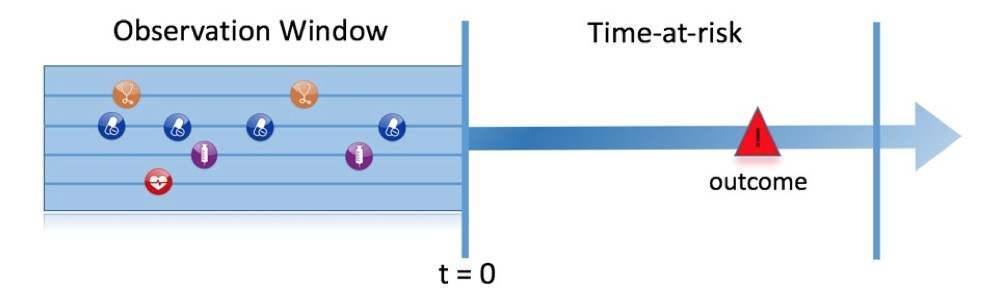
\includegraphics{Figure1.png}
\caption{The prediction problem}
\end{figure}

As shown in Figure 2, to define a prediction problem we have to define
t=0 by a Target Cohort (T), the outcome we like to predict by an outcome
cohort (O), and the time at risk (TAR). Furthermore, we have to make
design choices for the model we like to develop.

\begin{figure}
\centering
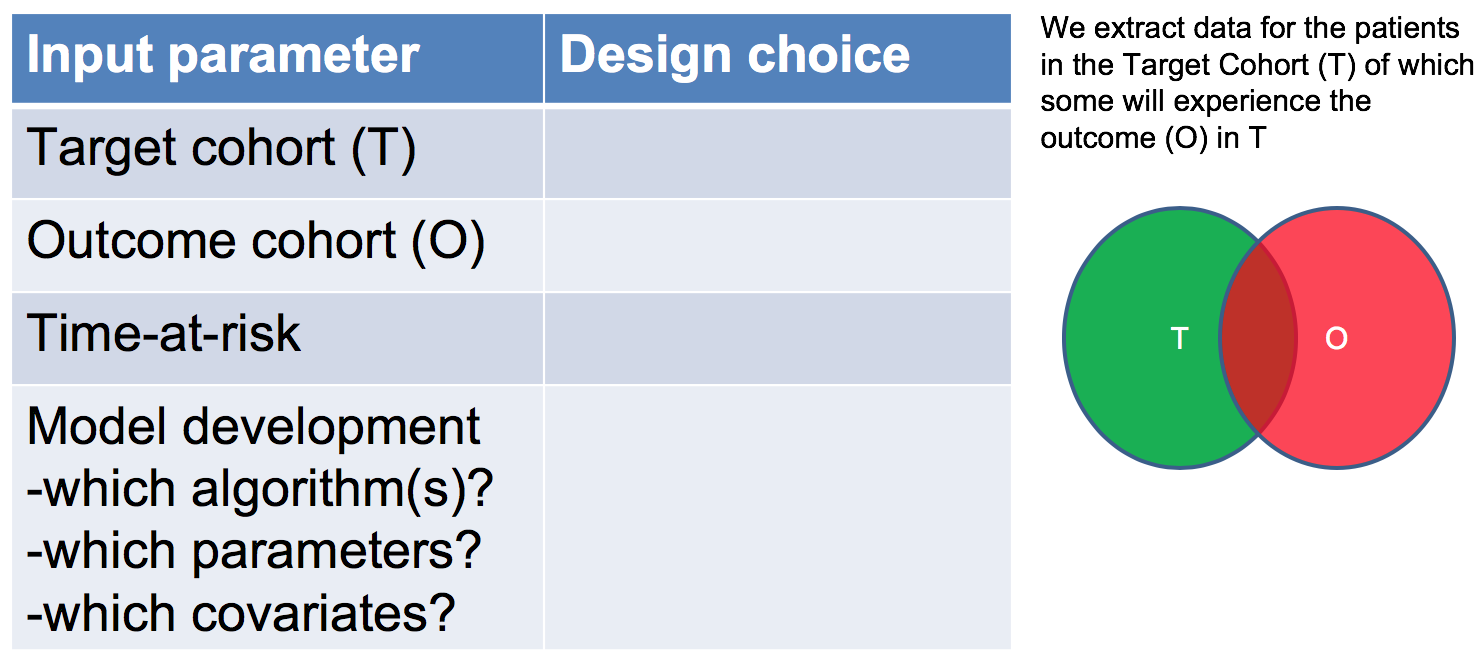
\includegraphics{studydesign.png}
\caption{Design choices}
\end{figure}

This framework works for all type of prediction problems, for example
those presented in Figure 3.

\begin{figure}
\centering
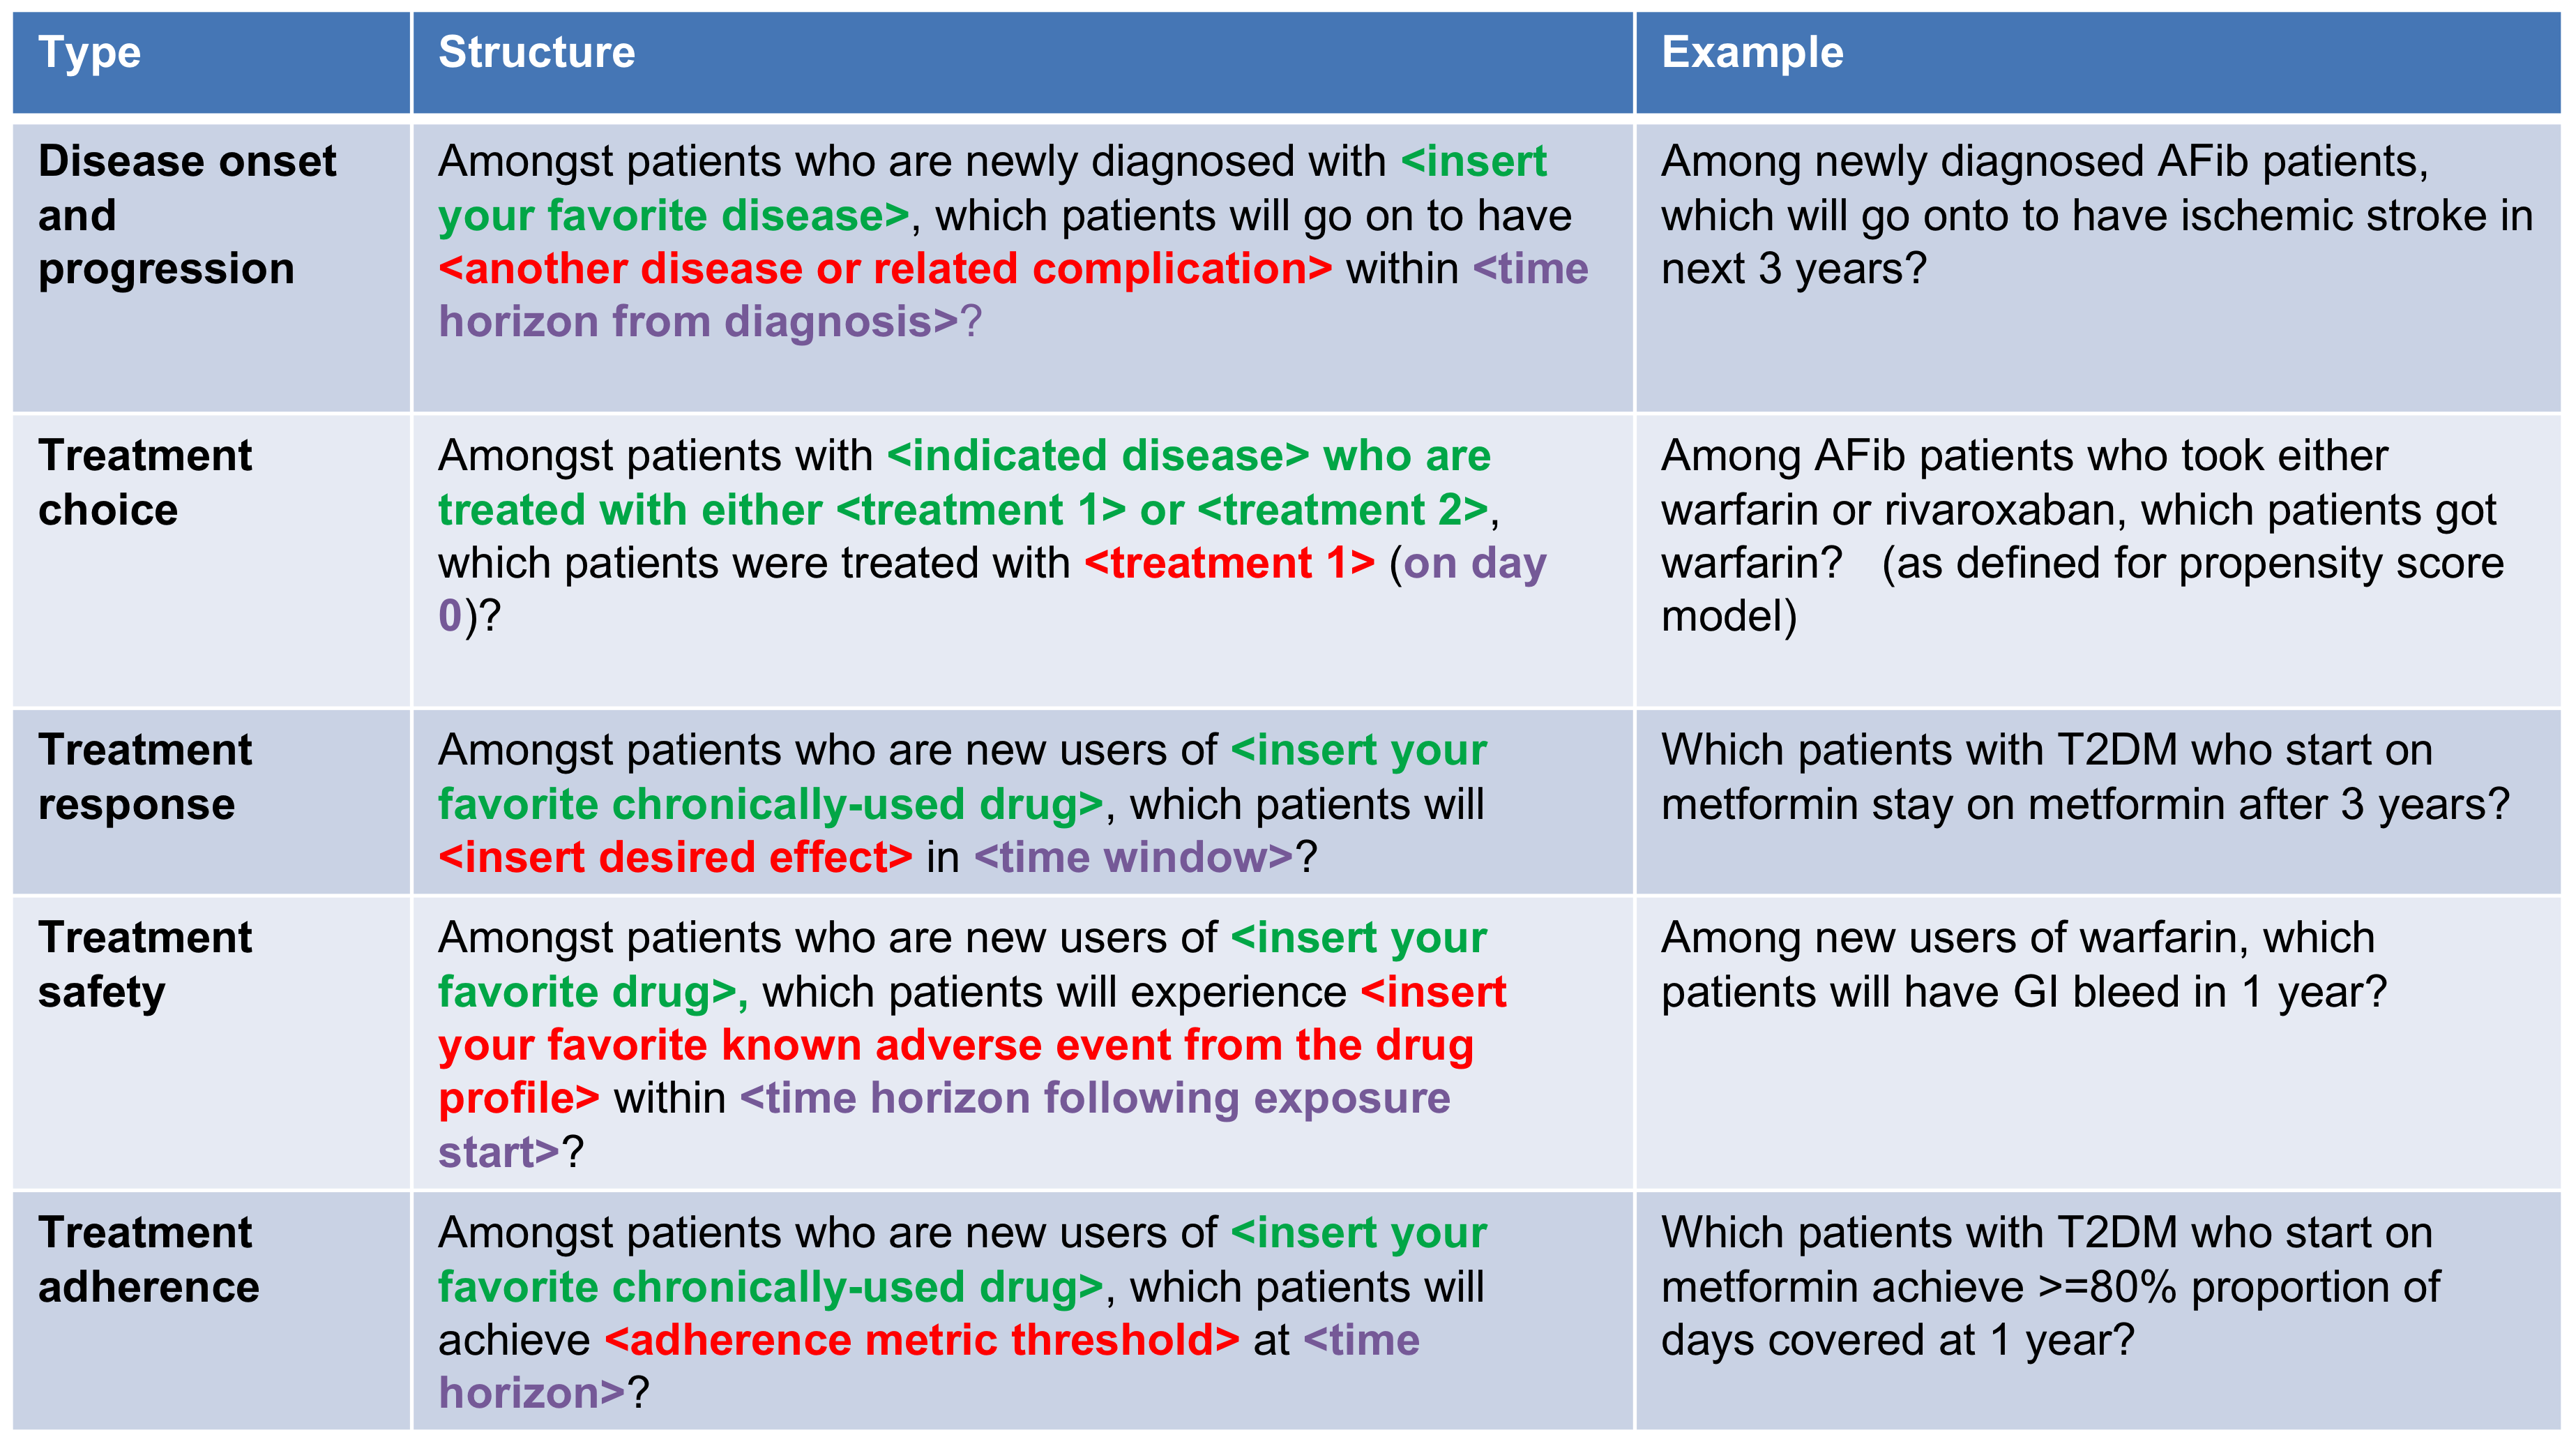
\includegraphics{problems.png}
\caption{Examples of prediction problems}
\end{figure}

This vignette describes how you can use the
\texttt{PatientLevelPrediction} package to build patient-level
predictive models. The package enables data extraction, model building,
and model evaluation using data from databases that are translated into
the Observational Medical Outcomes Partnership Common Data Model (OMOP
CDM). In this vignette we assume you have installed the package
correctly using the
\href{https://github.com/OHDSI/PatientLevelPrediction/blob/master/inst/doc/InstallationGuide.pdf}{InstallationGuide}.

To guide you through the process of model building and validation we
will use the ``Disease onset and progression'' type as an example.

\newpage

\section{Definition of the Prediction
Problem}\label{definition-of-the-prediction-problem}

Atrial fibrillation is a disease characterized by an irregular heart
rate that can cause poor blood flow. Patients with atrial fibrillation
are at increased risk of ischemic stroke. Anticoagulation is a
recommended prophylaxis treatment strategy for patients at high risk of
stroke, though the underuse of anticoagulants and persistent severity of
ischemic stroke represents a substantial unmet medical need. Various
strategies have been developed to predict risk of ischemic stroke in
patients with atrial fibrillation. CHADS2 (Gage JAMA 2001) was developed
as a risk score based on history of congestive heart failure,
hypertension, age\textgreater{}=75, diabetes and stroke. CHADS2 was
initially derived using Medicare claims data, where it achieved good
discrimination (AUC=0.82). However, subsequent external validation
studies revealed the CHADS2 had substantially lower predictive accuracy
(Keogh Thromb Haemost 2011). Subsequent stroke risk calculators have
been developed and evaluated, including the extension of CHADS2Vasc. The
management of atrial fibrillation has evolved substantially over the
last decade, for various reasons that include the introduction of novel
oral anticoagulants. With these innovations has come a renewed interest
in greater precision medicine for stroke prevention.

We will apply the PatientLevelPrediction package to observational
healthcare data to address the following patient-level prediction
question: Amongst patients who are newly diagnosed with Atrial
Fibrillation, which patients will go on to have Ischemic Stroke within 3
years?

We will define `patients who are newly diagnosed with Atrial
Fibrillation' as the first condition record of cardiac arrhythmia, which
is followed by another cardiac arrhythmia condition record, at least two
drug records for a drug used to treat arrhythmias, or a procedure to
treat arrhythmias. We will define `Ischemic stroke events' as ischemic
stroke condition records during an inpatient or ER visit; successive
records with \textgreater{} 180 day gap are considered independent
episodes.

\section{Data extraction}\label{data-extraction}

The \texttt{PatientLevelPrediction} package requires longitudinal
observational healthcare data in the OMOP Common Data Model format. We
will now explain how to connect to the server and how the generate the
Target (T=Atrial Fibrillation) and outcome cohort (O=Stroke).

\subsection{Configuring the connection to the
server}\label{configuring-the-connection-to-the-server}

First we need to tell R how to connect to the server.
\texttt{PatientLevelPrediction} uses the \texttt{DatabaseConnector}
package, which provides the \texttt{createConnectionDetails} function.
Type \texttt{?createConnectionDetails} for the specific settings
required for the various database management systems (DBMS). For
example, one might connect to a PostgreSQL database using this code:

\begin{Shaded}
\begin{Highlighting}[]
\NormalTok{connectionDetails <-}\StringTok{ }\KeywordTok{createConnectionDetails}\NormalTok{(}\DataTypeTok{dbms =} \StringTok{"postgresql"}\NormalTok{, }
                                             \DataTypeTok{server =} \StringTok{"localhost/ohdsi"}\NormalTok{, }
                                             \DataTypeTok{user =} \StringTok{"joe"}\NormalTok{, }
                                             \DataTypeTok{password =} \StringTok{"supersecret"}\NormalTok{)}

\NormalTok{cdmDatabaseSchema <-}\StringTok{ "my_cdm_data"}
\NormalTok{cohortsDatabaseSchema <-}\StringTok{ "my_results"}
\NormalTok{cdmVersion <-}\StringTok{ "5"}
\end{Highlighting}
\end{Shaded}

The last three lines define the \texttt{cdmDatabaseSchema} and
\texttt{cohortsDatabaseSchema} variables, as well as the CDM version. We
will use these later to tell R where the data in CDM format live, where
we want to create the cohorts of interest, and what version CDM is used.
Note that for Microsoft SQL Server, databaseschemas need to specify both
the database and the schema, so for example
\texttt{cdmDatabaseSchema\ \textless{}-\ "my\_cdm\_data.dbo"}.

\subsection{Preparing the cohort and outcome of
interest}\label{preparing-the-cohort-and-outcome-of-interest}

First we need to define the cohort of persons for which we want to
perform the prediction and we need to define the outcome we want to
predict. These cohorts are provided as data in a table on the server
that has the same structure as the `cohort' table in the OMOP CDM,
meaning it should have the following columns:

\begin{itemize}
\tightlist
\item
  \texttt{cohort\_definition\_id}, a unique identifier for
  distinguishing between different types of cohorts, e.g.~cohorts of
  interest and outcome cohorts.
\item
  \texttt{subject\_id}, a unique identifier corresponding to the
  \texttt{person\_id} in the CDM.
\item
  \texttt{cohort\_start\_date}, the start of the time period where we
  wish to predict the occurrence of the outcome.
\item
  \texttt{cohort\_end\_date}, which can be used to determine the end of
  the prediction window. Can be set equal to the
  \texttt{cohort\_start\_date} for outcomes.
\end{itemize}

The observational and health data sciences \& informatics (OHDSI)
community has developed a tool named ATLAS which can be used to create
cohorts based on inclusion criteria. We can also write custom SQL
statements against the CDM. Both methods are described below.

\subsubsection{Cohort creation using
ATLAS}\label{cohort-creation-using-atlas}

!!!!! TO BE UPDATED WITH COHORT FIGURES AND TEXT OF PATRICK

\begin{figure}
\centering
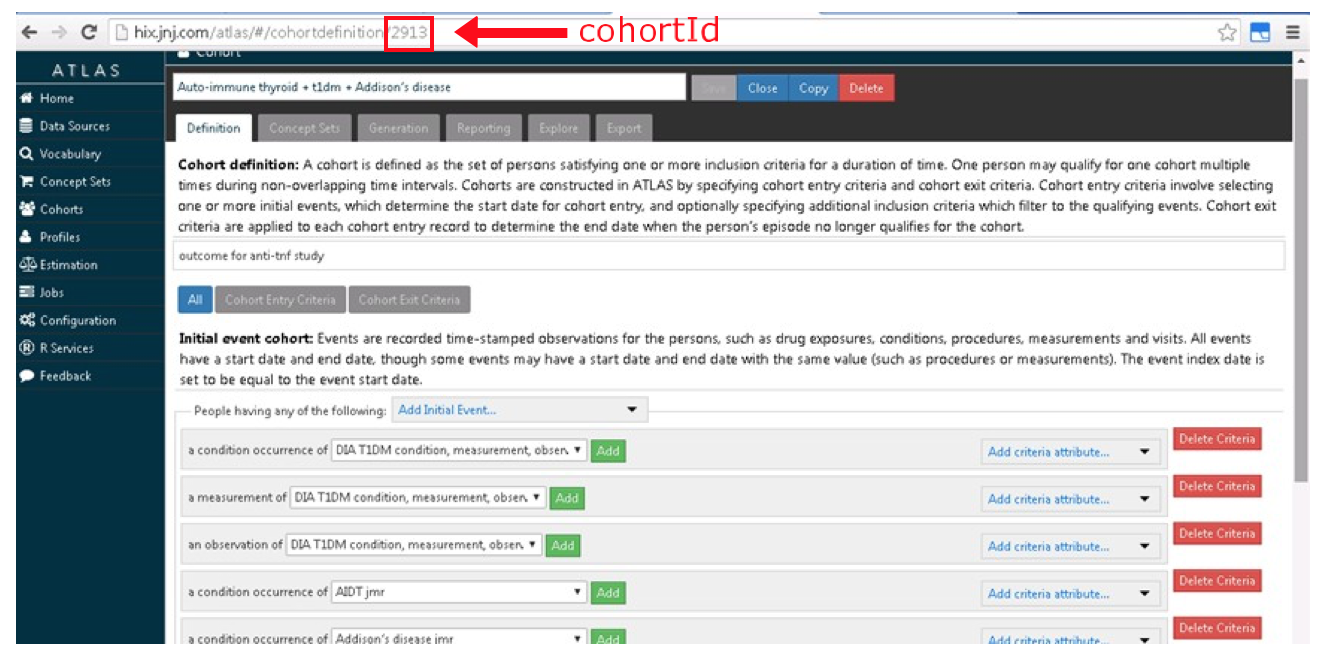
\includegraphics{Figure2.png}
\caption{Cohort creation using ATLAS}
\end{figure}

ATLAS as shown in Figure 2 allows you to define cohorts interactively by
specifying cohort entry and cohort exit criteria. Cohort entry criteria
involce selecting one or more initial events, which determine the start
date for cohort entry, and optionally specifying additional inclusion
criteria which filter to the qualifying events. Cohort exit criteria are
applied to each cohort entry record to determine the end date when the
person's episode no longer qualifies for the cohort. For the outcome
cohort the end date is less relevant. More details on the use of ATLAS
can be found on the OHDSI wiki pages.

When a cohort is created in ATLAS the cohortid is needed to extract the
data in R. The cohortid can be found in the link as shown in Figure 2.

\subsubsection{Custom cohort creation}\label{custom-cohort-creation}

!!!!! TO BE UPDATED WITH SQL AND TEXT OF PATRICK

It is also possible to create cohorts without the use of ATLAS. Using
custom cohort code (SQL) you can make more advanced cohorts if needed.

For our example study, we need to create the cohort of diabetics that
have been hospitalized and have a minimum amount of observation time
available before and after the hospitalization. We also need to define
re-hospitalizations, which we define as any hospitalizations occurring
after the original hospitalization.

For this purpose we have created a file called
\emph{HospitalizationCohorts.sql} with the following contents:

\begin{Shaded}
\begin{Highlighting}[]
\CommentTok{/***********************************}
\CommentTok{File HospitalizationCohorts.sql }
\CommentTok{***********************************/}
\KeywordTok{IF}\NormalTok{ OBJECT_ID(}\StringTok{'@resultsDatabaseSchema.rehospitalization'}\NormalTok{, }\StringTok{'U'}\NormalTok{) }\KeywordTok{IS} \KeywordTok{NOT} \KeywordTok{NULL}
\KeywordTok{DROP} \KeywordTok{TABLE}\NormalTok{ @resultsDatabaseSchema.rehospitalization;}

\KeywordTok{SELECT}\NormalTok{ visit_occurrence.person_id }\KeywordTok{AS}\NormalTok{ subject_id,}
\FunctionTok{MIN}\NormalTok{(visit_start_date) }\KeywordTok{AS}\NormalTok{ cohort_start_date,}
\NormalTok{DATEADD(}\DataTypeTok{DAY}\NormalTok{, @post_time, }\FunctionTok{MIN}\NormalTok{(visit_start_date)) }\KeywordTok{AS}\NormalTok{ cohort_end_date,}
\DecValTok{1} \KeywordTok{AS}\NormalTok{ cohort_definition_id}
\KeywordTok{INTO}\NormalTok{ @resultsDatabaseSchema.rehospitalization}
\KeywordTok{FROM}\NormalTok{ @cdmDatabaseSchema.visit_occurrence}
\KeywordTok{INNER} \KeywordTok{JOIN}\NormalTok{ @cdmDatabaseSchema.observation_period}
\KeywordTok{ON}\NormalTok{ visit_occurrence.person_id = observation_period.person_id}
\KeywordTok{INNER} \KeywordTok{JOIN}\NormalTok{ @cdmDatabaseSchema.condition_occurrence}
\KeywordTok{ON}\NormalTok{ condition_occurrence.person_id = visit_occurrence.person_id }
\KeywordTok{WHERE}\NormalTok{ visit_concept_id }\KeywordTok{IN}\NormalTok{ (}\DecValTok{9201}\NormalTok{, }\DecValTok{9203}\NormalTok{)}
\KeywordTok{AND}\NormalTok{ DATEDIFF(}\DataTypeTok{DAY}\NormalTok{, observation_period_start_date, visit_start_date) > @pre_time}
\KeywordTok{AND}\NormalTok{ visit_start_date > observation_period_start_date}
\KeywordTok{AND}\NormalTok{ DATEDIFF(}\DataTypeTok{DAY}\NormalTok{, visit_start_date, observation_period_end_date) > @post_time}
\KeywordTok{AND}\NormalTok{ visit_start_date < observation_period_end_date}
\KeywordTok{AND}\NormalTok{ DATEDIFF(}\DataTypeTok{DAY}\NormalTok{, condition_start_date, visit_start_date) > @pre_time}
\KeywordTok{AND}\NormalTok{ condition_start_date <= visit_start_date}
\KeywordTok{AND}\NormalTok{ condition_concept_id }\KeywordTok{IN}\NormalTok{ (}
\KeywordTok{SELECT}\NormalTok{ descendant_concept_id }
\KeywordTok{FROM}\NormalTok{ @cdmDatabaseSchema.concept_ancestor }
\KeywordTok{WHERE}\NormalTok{ ancestor_concept_id = }\DecValTok{201826}\NormalTok{) }\CommentTok{/* Type 2 DM */}
\KeywordTok{GROUP} \KeywordTok{BY}\NormalTok{ visit_occurrence.person_id;}

\KeywordTok{INSERT} \KeywordTok{INTO}\NormalTok{ @resultsDatabaseSchema.rehospitalization}
\KeywordTok{SELECT}\NormalTok{ visit_occurrence.person_id }\KeywordTok{AS}\NormalTok{ subject_id,}
\NormalTok{visit_start_date }\KeywordTok{AS}\NormalTok{ cohort_start_date,}
\NormalTok{visit_end_date }\KeywordTok{AS}\NormalTok{ cohort_end_date,}
\DecValTok{2} \KeywordTok{AS}\NormalTok{ cohort_definition_id}
\KeywordTok{FROM}\NormalTok{ @resultsDatabaseSchema.rehospitalization}
\KeywordTok{INNER} \KeywordTok{JOIN}\NormalTok{ @cdmDatabaseSchema.visit_occurrence}
\KeywordTok{ON}\NormalTok{ visit_occurrence.person_id = rehospitalization.subject_id}
\KeywordTok{WHERE}\NormalTok{ visit_concept_id }\KeywordTok{IN}\NormalTok{ (}\DecValTok{9201}\NormalTok{, }\DecValTok{9203}\NormalTok{)}
\KeywordTok{AND}\NormalTok{ visit_start_date > cohort_start_date}
\KeywordTok{AND}\NormalTok{ visit_start_date <= cohort_end_date}
\KeywordTok{AND}\NormalTok{ cohort_definition_id = }\DecValTok{1}\NormalTok{;}
\end{Highlighting}
\end{Shaded}

This is parameterized SQL which can be used by the \texttt{SqlRender}
package. We use parameterized SQL so we do not have to pre-specify the
names of the CDM and result schemas. That way, if we want to run the SQL
on a different schema, we only need to change the parameter values; we
do not have to change the SQL code. By also making use of translation
functionality in \texttt{SqlRender}, we can make sure the SQL code can
be run in many different environments.

\begin{Shaded}
\begin{Highlighting}[]
\KeywordTok{library}\NormalTok{(SqlRender)}
\NormalTok{sql <-}\StringTok{ }\KeywordTok{readSql}\NormalTok{(}\StringTok{"HospitalizationCohorts.sql"}\NormalTok{)}
\NormalTok{sql <-}\StringTok{ }\KeywordTok{renderSql}\NormalTok{(sql,}
\DataTypeTok{cdmDatabaseSchema =}\NormalTok{ cdmDatabaseSchema,}
\DataTypeTok{cohortsDatabaseSchema =}\NormalTok{ cohortsDatabaseSchema,}
\DataTypeTok{post_time =} \DecValTok{30}\NormalTok{,}
\DataTypeTok{pre_time =} \DecValTok{365}\NormalTok{)}\OperatorTok{$}\NormalTok{sql}
\NormalTok{sql <-}\StringTok{ }\KeywordTok{translateSql}\NormalTok{(sql, }\DataTypeTok{targetDialect =}\NormalTok{ connectionDetails}\OperatorTok{$}\NormalTok{dbms)}\OperatorTok{$}\NormalTok{sql}

\NormalTok{connection <-}\StringTok{ }\KeywordTok{connect}\NormalTok{(connectionDetails)}
\KeywordTok{executeSql}\NormalTok{(connection, sql)}
\end{Highlighting}
\end{Shaded}

In this code, we first read the SQL from the file into memory. In the
next line, we replace four parameter names with the actual values. We
then translate the SQL into the dialect appropriate for the DBMS we
already specified in the \texttt{connectionDetails}. Next, we connect to
the server, and submit the rendered and translated SQL.

If all went well, we now have a table with the events of interest. We
can see how many events per type:

\begin{Shaded}
\begin{Highlighting}[]
\NormalTok{sql <-}\StringTok{ }\KeywordTok{paste}\NormalTok{(}\StringTok{"SELECT cohort_definition_id, COUNT(*) AS count"}\NormalTok{,}
\StringTok{"FROM @cohortsDatabaseSchema.rehospitalization"}\NormalTok{,}
\StringTok{"GROUP BY cohort_definition_id"}\NormalTok{)}
\NormalTok{sql <-}\StringTok{ }\KeywordTok{renderSql}\NormalTok{(sql, }\DataTypeTok{cohortsDatabaseSchema =}\NormalTok{ cohortsDatabaseSchema)}\OperatorTok{$}\NormalTok{sql}
\NormalTok{sql <-}\StringTok{ }\KeywordTok{translateSql}\NormalTok{(sql, }\DataTypeTok{targetDialect =}\NormalTok{ connectionDetails}\OperatorTok{$}\NormalTok{dbms)}\OperatorTok{$}\NormalTok{sql}

\KeywordTok{querySql}\NormalTok{(connection, sql)}
\end{Highlighting}
\end{Shaded}

\begin{verbatim}
##   cohort_definition_id  count
## 1                    1 527616
## 2                    2 221555
\end{verbatim}

\subsection{Extracting the data from the
server}\label{extracting-the-data-from-the-server}

Now we can tell \texttt{PatientLevelPrediction} to extract all necessary
data for our analysis. This is done using the
\texttt{FeatureExtractionPackage} available at
\url{https://github.com/OHDSI/FeatureExtration}. In short the
FeatureExtractionPackage allows you to specify which features
(covariates) need to be extracted, e.g.~all conditions and drug
exposures. It also supports the creation of custom covariates. For more
detailed information on the FeatureExtraction package see its vignettes.

\begin{Shaded}
\begin{Highlighting}[]
\NormalTok{covariateSettings <-}\StringTok{ }\KeywordTok{createCovariateSettings}\NormalTok{(}\DataTypeTok{useDemographicsGender =} \OtherTok{TRUE}\NormalTok{,}
\DataTypeTok{useDemographicsAge =} \OtherTok{TRUE}\NormalTok{, }\DataTypeTok{useDemographicsAgeGroup =} \OtherTok{TRUE}\NormalTok{,}
\DataTypeTok{useDemographicsRace =} \OtherTok{TRUE}\NormalTok{, }\DataTypeTok{useDemographicsEthnicity =} \OtherTok{TRUE}\NormalTok{,}
\DataTypeTok{useConditionOccurrenceLongTerm =} \OtherTok{TRUE}\NormalTok{,}
\DataTypeTok{useDrugExposureLongTerm =} \OtherTok{TRUE}\NormalTok{,}
\DataTypeTok{useProcedureOccurrenceLongTerm =} \OtherTok{TRUE}\NormalTok{,}
\DataTypeTok{useMeasurementLongTerm =} \OtherTok{TRUE}\NormalTok{,}
\DataTypeTok{useObservationLongTerm =} \OtherTok{TRUE}\NormalTok{,}
\DataTypeTok{useDistinctConditionCountLongTerm =}\OtherTok{TRUE}\NormalTok{,}
\DataTypeTok{useVisitCountLongTerm =} \OtherTok{TRUE}\NormalTok{, }
\DataTypeTok{longTermStartDays =} \OperatorTok{-}\DecValTok{365}\NormalTok{,}
\DataTypeTok{endDays =} \OperatorTok{-}\DecValTok{1}\NormalTok{)}
\end{Highlighting}
\end{Shaded}

The final step for extracting the data is to run the \texttt{getPlpData}
function and input the connection details, the database schema where the
cohorts are stored, the cohort definition ids for the cohort and
outcome, and the washoutPeriod which is the minimum number of days prior
to cohort index date that the person must have been observed to be
included into the data, and finally input the previously constructed
covariate settings.

\begin{Shaded}
\begin{Highlighting}[]
\NormalTok{plpData <-}\StringTok{ }\KeywordTok{getPlpData}\NormalTok{(}\DataTypeTok{connectionDetails =}\NormalTok{ connectionDetails,}
\DataTypeTok{cdmDatabaseSchema =}\NormalTok{ cdmDatabaseSchema,}
\DataTypeTok{oracleTempSchema =}\NormalTok{ oracleTempSchema,}
\DataTypeTok{cohortDatabaseSchema =}\NormalTok{ cohortsDatabaseSchema,}
\DataTypeTok{cohortTable =} \StringTok{"rehospitalization"}\NormalTok{,}
\DataTypeTok{cohortId =} \DecValTok{1}\NormalTok{,}
\DataTypeTok{washoutPeriod =} \DecValTok{183}\NormalTok{,}
\DataTypeTok{covariateSettings =}\NormalTok{ covariateSettings,}
\DataTypeTok{outcomeDatabaseSchema =}\NormalTok{ cohortsDatabaseSchema,}
\DataTypeTok{outcomeTable =} \StringTok{"rehospitalization"}\NormalTok{,}
\DataTypeTok{outcomeIds =} \DecValTok{2}\NormalTok{,}
\DataTypeTok{cdmVersion =}\NormalTok{ cdmVersion)}
\end{Highlighting}
\end{Shaded}

Note that if the cohorts are created in ATLAS its corresponding cohort
database schema needs to be selected. There are many additional
parameters for the \texttt{getPlpData} function which are all documented
in the \texttt{PatientLevelPrediction} manual. The resulting
\texttt{plpData} object uses the package \texttt{ff} to store
information in a way that ensures R does not run out of memory, even
when the data are large.

\subsection{Saving the data to file}\label{saving-the-data-to-file}

Creating the \texttt{plpData} object can take considerable computing
time, and it is probably a good idea to save it for future sessions.
Because \texttt{plpData} uses \texttt{ff}, we cannot use R's regular
save function. Instead, we'll have to use the \texttt{savePlpData()}
function:

\begin{Shaded}
\begin{Highlighting}[]
\KeywordTok{savePlpData}\NormalTok{(plpData, }\StringTok{"stroke_in_af_data"}\NormalTok{)}
\end{Highlighting}
\end{Shaded}

We can use the \texttt{loadPlpData()} function to load the data in a
future session.

\section{Applying additional inclusion
criteria}\label{applying-additional-inclusion-criteria}

To completely define the prediction problem the final study population
is obtained by applying additional constraints on the two earlier
defined cohorts, e.g., a minumim time at risk can be enforced
(\texttt{requireTimeAtRisk,\ minTimeAtRisk}). In this step it is also
possible to redefine the risk window based on the at-risk cohort. For
example, if we like the risk window to start 30 days after the at-risk
cohort start and end a year later we can set
\texttt{riskWindowStart\ =\ 30} and \texttt{riskWindowEnd\ =\ 365}. In
some cases the risk window needs to start at the cohort end date. This
can be achieved by setting \texttt{addExposureToStart\ =\ TRUE} which
adds the cohort (exposure) time to the start date.

In the example below a final population is created using an additional
constraint on the washout period, removal of patients with prior
outcomes in the year before, and a time at risk definition.

\begin{Shaded}
\begin{Highlighting}[]
\NormalTok{population <-}\StringTok{ }\KeywordTok{createStudyPopulation}\NormalTok{(plpData, }
\DataTypeTok{outcomeId =} \DecValTok{2}\NormalTok{, }
\DataTypeTok{includeAllOutcomes =} \OtherTok{TRUE}\NormalTok{, }
\DataTypeTok{firstExposureOnly =} \OtherTok{TRUE}\NormalTok{, }
\DataTypeTok{washoutPeriod =} \DecValTok{365}\NormalTok{, }
\DataTypeTok{removeSubjectsWithPriorOutcome =} \OtherTok{TRUE}\NormalTok{, }
\DataTypeTok{priorOutcomeLookback =} \DecValTok{365}\NormalTok{,}
\DataTypeTok{riskWindowStart =} \DecValTok{1}\NormalTok{,}
\DataTypeTok{requireTimeAtRisk =} \OtherTok{FALSE}\NormalTok{,}
\DataTypeTok{riskWindowEnd =} \DecValTok{365}\NormalTok{)}
\end{Highlighting}
\end{Shaded}

Note that some of these constraints could also already be applied in the
cohort creation step, however, the \texttt{createStudyPopulation}
function allows you do sensitivity analyses more easily on the already
extracted plpData from the database.

\newpage

\section{Model Development}\label{model-development}

\subsection{Selecting the algorithm}\label{selecting-the-algorithm}

We see the selection of the best algorithm for a certain prediction
problem as an emperical question, i.e.~you need to let the data speak
for itself and try different approaches to find the best. There is no
algorithm that will work best for all problems (no free lunch). In our
package we therefore aim to implement many algorithms. Furthermore, we
made the system modular so you can add your own custom algorithms as
described in more detail in the
\href{Link\%20to\%20be\%20added}{AddingCustomAlgorithms} vignette.

Our package currently contains the following algorithms:

\begin{longtable}[]{@{}lll@{}}
\toprule
\begin{minipage}[b]{0.12\columnwidth}\raggedright\strut
Algorihm\strut
\end{minipage} & \begin{minipage}[b]{0.55\columnwidth}\raggedright\strut
Description\strut
\end{minipage} & \begin{minipage}[b]{0.25\columnwidth}\raggedright\strut
Hyper-parameters\strut
\end{minipage}\tabularnewline
\midrule
\endhead
\begin{minipage}[t]{0.12\columnwidth}\raggedright\strut
Regularized Logistic Regression\strut
\end{minipage} & \begin{minipage}[t]{0.55\columnwidth}\raggedright\strut
Lasso logistic regression belongs to the family of generalized linear
models, where a linear combination of the variables is learned and
finally a logistic function maps the linear combination to a value
between 0 and 1. The lasso regularization adds a cost based on model
complexity to the objective function when training the model. This cost
is the sum of the absolute values of the linear combination of the
coefficients. The model automatically performs feature selection by
minimizing this cost. We use the Cyclic coordinate descent for logistic,
Poisson and survival analysis (Cyclops) package to perform large-scale
regularized logistic regression:
\url{https://github.com/OHDSI/Cyclops}\strut
\end{minipage} & \begin{minipage}[t]{0.25\columnwidth}\raggedright\strut
var (starting variance), seed\strut
\end{minipage}\tabularnewline
\begin{minipage}[t]{0.12\columnwidth}\raggedright\strut
Gradient boosting machines\strut
\end{minipage} & \begin{minipage}[t]{0.55\columnwidth}\raggedright\strut
Gradient boosting machines is a boosting ensemble technique and in our
framework it combines multiple decision trees. Boosting works by
iteratively adding decision trees but adds more weight to the
data-points that are misclassified by prior decision trees in the cost
function when training the next tree. We use Extreme Gradient Boosting,
which is an efficient implementation of the gradient boosting framework
implemented in the xgboost R package available from CRAN.\strut
\end{minipage} & \begin{minipage}[t]{0.25\columnwidth}\raggedright\strut
ntree (number of trees), max depth (max levels in tree), min rows
(minimum data points in in node), learning rate, seed\strut
\end{minipage}\tabularnewline
\begin{minipage}[t]{0.12\columnwidth}\raggedright\strut
Random forest\strut
\end{minipage} & \begin{minipage}[t]{0.55\columnwidth}\raggedright\strut
Random forest is a bagging ensemble technique that combines multiple
decision trees. The idea behind bagging is to reduce the likelihood of
overfitting, by using weak classifiers, but combining multiple diverse
weak classifiers into a strong classifier. Random forest accomplishes
this by training multiple decision trees but only using a subset of the
variables in each tree and the subset of variables differ between trees.
Our packages uses the sklearn learn implementation of Random Forest in
python.\strut
\end{minipage} & \begin{minipage}[t]{0.25\columnwidth}\raggedright\strut
mtry (number of features in each tree),ntree (number of trees), maxDepth
(max levels in tree), minRows (minimum data points in in node),balance
(balance class labels), seed\strut
\end{minipage}\tabularnewline
\begin{minipage}[t]{0.12\columnwidth}\raggedright\strut
K-nearest neighbors\strut
\end{minipage} & \begin{minipage}[t]{0.55\columnwidth}\raggedright\strut
K-nearest neighbors (KNN) is an algorithm that uses some metric to find
the K closest labelled data-points, given the specified metric, to a new
unlabelled data-point. The prediction of the new data-points is then the
most prevalent class of the K-nearest labelled data-points. There is a
sharing limitation of KNN, as the model requires labelled data to
perform the prediction on new data, and it is often not possible to
share this data across data sites.We included the BigKnn classifier
developed in OHDSI which is a large scale k-nearest neighbor classifier
using the Lucene search engine:
\url{https://github.com/OHDSI/BigKnn}\strut
\end{minipage} & \begin{minipage}[t]{0.25\columnwidth}\raggedright\strut
k (number of neighbours),weighted (weight by inverse frequency)\strut
\end{minipage}\tabularnewline
\begin{minipage}[t]{0.12\columnwidth}\raggedright\strut
Naive Bayes\strut
\end{minipage} & \begin{minipage}[t]{0.55\columnwidth}\raggedright\strut
To add\strut
\end{minipage} & \begin{minipage}[t]{0.25\columnwidth}\raggedright\strut
none\strut
\end{minipage}\tabularnewline
\begin{minipage}[t]{0.12\columnwidth}\raggedright\strut
AdaBoost\strut
\end{minipage} & \begin{minipage}[t]{0.55\columnwidth}\raggedright\strut
AdaBoost is a boosting ensemble technique. Boosting works by iteratively
adding decision trees but adds more weight to the data-points that are
misclassified by prior decision trees in the cost function when training
the next tree.We use the sklearn ``AdaboostClassifier'' implementation
in Python.\strut
\end{minipage} & \begin{minipage}[t]{0.25\columnwidth}\raggedright\strut
nEstimators (the maximum number of estimators at which boosting is
terminated), learningRate (learning rate shrinks the contribution of
each classifier by learning\_rate. There is a trade-off between
learningRate and nEstimators)\strut
\end{minipage}\tabularnewline
\begin{minipage}[t]{0.12\columnwidth}\raggedright\strut
Decision Tree\strut
\end{minipage} & \begin{minipage}[t]{0.55\columnwidth}\raggedright\strut
A decision tree is a classifier that partitions the variable space using
individual tests selected using a greedy approach. It aims to find
partitions that have the highest information gain to separate the
classes. The decision tree can easily overfit by enabling a large number
of partitions (tree depth) and often needs some regularization (e.g.,
pruning or specifying hyper-parameters that limit the complexity of the
model). We use the sklearn ``DecisionTreeClassifier'' implementation in
Python.\strut
\end{minipage} & \begin{minipage}[t]{0.25\columnwidth}\raggedright\strut
maxDepth (the maximum depth of the tree),
minSamplesSplit,minSamplesLeaf, minImpuritySplit (threshold for early
stopping in tree growth. A node will split if its impurity is above the
threshold, otherwise it is a leaf.), seed,classWeight (``Balance''" or
``None'')\strut
\end{minipage}\tabularnewline
\begin{minipage}[t]{0.12\columnwidth}\raggedright\strut
Multilayer Perception\strut
\end{minipage} & \begin{minipage}[t]{0.55\columnwidth}\raggedright\strut
Neural networks contain multiple layers that weight their inputs using
an non-linear function. The first layer is the input layer, the last
layer is the output layer the between are the hidden layers. Neural
networks are generally trained using feed forward back-propagation. This
is when you go through the network with a data-point and calculate the
error between the true label and predicted label, then go backwards
through the network and update the linear function weights based on the
error. This can also be performed as a batch, where multiple data-points
are fee\strut
\end{minipage} & \begin{minipage}[t]{0.25\columnwidth}\raggedright\strut
size (the number of hidden nodes), alpha (the l2 regularisation),
seed\strut
\end{minipage}\tabularnewline
\begin{minipage}[t]{0.12\columnwidth}\raggedright\strut
Deep Learning\strut
\end{minipage} & \begin{minipage}[t]{0.55\columnwidth}\raggedright\strut
Deep learning such as deep nets, convolutional neural networks or
recurrent neural networks are similar to a neural network but have
multiple hidden layers that aim to learn latent representations useful
for prediction. In the seperate BuildingDeepLearningModels vignette we
describe these models and hyper-parameters in more detail\strut
\end{minipage} & \begin{minipage}[t]{0.25\columnwidth}\raggedright\strut
\strut
\end{minipage}\tabularnewline
\bottomrule
\end{longtable}

In the settings function of the algorithms the user can specify a list
of eligible values for each hyper-parameter. All possible combinations
of the hyper-parameters are included in a so-called grid search using
cross-validation on the training set. If a user does not specify any
value then the default value is used instead.

For example, if we use the following settings for the
gradientBoostingMachine: ntrees=c(100,200), maxDepth=4 the grid search
will apply the gradient boosting machine algorithm with ntrees=100 and
maxDepth=4 plus the default settings for other hyper-parameters and
ntrees=200 and maxDepth=4 plus the default settings for other
hyper-parameters. The hyper-parameters that lead to the
bestcross-validation performance will then be chosen for the final
model. For our problem we choose to build a logistic regression model
with the default hyper-parameters.

\begin{Shaded}
\begin{Highlighting}[]
\NormalTok{lrModel <-}\StringTok{ }\KeywordTok{setLassoLogisticRegression}\NormalTok{()}
\end{Highlighting}
\end{Shaded}

\subsection{Model training}\label{model-training}

The \texttt{runPlP} function uses the population, \texttt{plpData}, and
model settings to train and evaluate the model. Because evaluation using
the same data on which the model was built can lead to overfitting, one
uses a train-test split of the data or cross-validation. This
functionaity is build in the \texttt{runPlP} function. We can use the
testSplit (person/time) and testFraction parameters to split the data in
a 75\%-25\% split and run the patient-level prediction pipeline:

\begin{Shaded}
\begin{Highlighting}[]
\NormalTok{lrResults <-}\StringTok{ }\KeywordTok{runPlp}\NormalTok{(population,plpData, }\DataTypeTok{modelSettings =}\NormalTok{ lrModel, }\DataTypeTok{testSplit =} \StringTok{'person'}\NormalTok{,  }
\DataTypeTok{testFraction =} \FloatTok{0.25}\NormalTok{, }\DataTypeTok{nfold =} \DecValTok{2}\NormalTok{)}
\end{Highlighting}
\end{Shaded}

Under the hood the package will now use the \texttt{Cyclops} package to
fit a large-scale regularized regression using 75\% of the data and will
evaluate the model on the remaining 25\%. A results data structure is
returned containing information about the model, its performance etc.

\subsection{Saving and loading}\label{saving-and-loading}

You can save and load the model using:

\begin{Shaded}
\begin{Highlighting}[]
\KeywordTok{savePlpModel}\NormalTok{(lrResults}\OperatorTok{$}\NormalTok{model, }\DataTypeTok{dirPath =} \KeywordTok{file.path}\NormalTok{(}\KeywordTok{getwd}\NormalTok{(), }\StringTok{"model"}\NormalTok{))}
\NormalTok{plpModel <-}\StringTok{ }\KeywordTok{loadPlpModel}\NormalTok{(}\KeywordTok{getwd}\NormalTok{(), }\StringTok{"model"}\NormalTok{)}
\end{Highlighting}
\end{Shaded}

You can save and load the full results structure using:

\begin{Shaded}
\begin{Highlighting}[]
\KeywordTok{savePlpResult}\NormalTok{(lrResults, }\DataTypeTok{location =} \KeywordTok{file.path}\NormalTok{(}\KeywordTok{getwd}\NormalTok{(), }\StringTok{"lr"}\NormalTok{))}
\NormalTok{lrResults <-}\StringTok{ }\KeywordTok{loadPlpResult}\NormalTok{(}\KeywordTok{file.path}\NormalTok{(}\KeywordTok{getwd}\NormalTok{(), }\StringTok{"lr"}\NormalTok{))}
\end{Highlighting}
\end{Shaded}

\newpage

\section{Model Evaluation}\label{model-evaluation}

The runPlp() function returns the trained model and the evaluation of
the model on the train/test sets.

You can also interactively view the results by running:
\texttt{viewPlp(runPlp=lrResults)}. This will generate a Shiny App in
which you can view all plots and performance measure created by the
framework as shown in the Figure below.

!!! TO BE REPLACE BY SHINY APP EXAMPLE OF PATRICK

To generate and save all the evaluation plots run the following code:

\begin{Shaded}
\begin{Highlighting}[]
\KeywordTok{plotPlp}\NormalTok{(lrResults, }\DataTypeTok{dirPath =} \KeywordTok{getwd}\NormalTok{())}
\end{Highlighting}
\end{Shaded}

The plots that are generated are described in more detail in the next
sections.

\newpage

\subsection{ROC plot}\label{roc-plot}

\begin{figure}
\centering
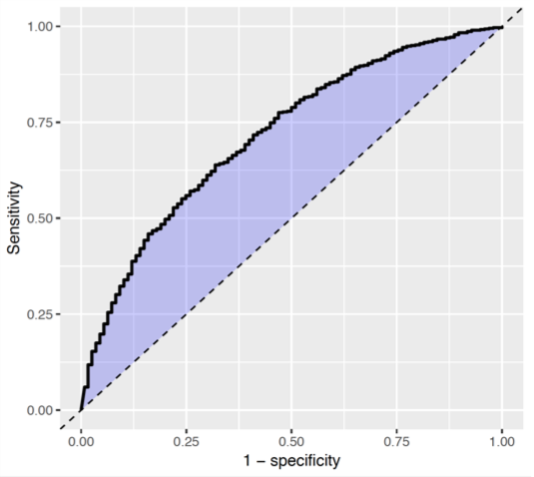
\includegraphics{sparseRoc.png}
\caption{Receiver Operator Plot}
\end{figure}

The ROC plot plots the sensitivity against 1-specificity on the test
set. The plot shows how well the model is able to discriminate between
the people with the outcome and those without. The dashed diagonal line
is the performance of a model that randomly assigns predictions. The
higher the area under the ROC plot the better the discrimination of the
model.

\newpage

\subsection{Calibration plot}\label{calibration-plot}

\begin{figure}
\centering
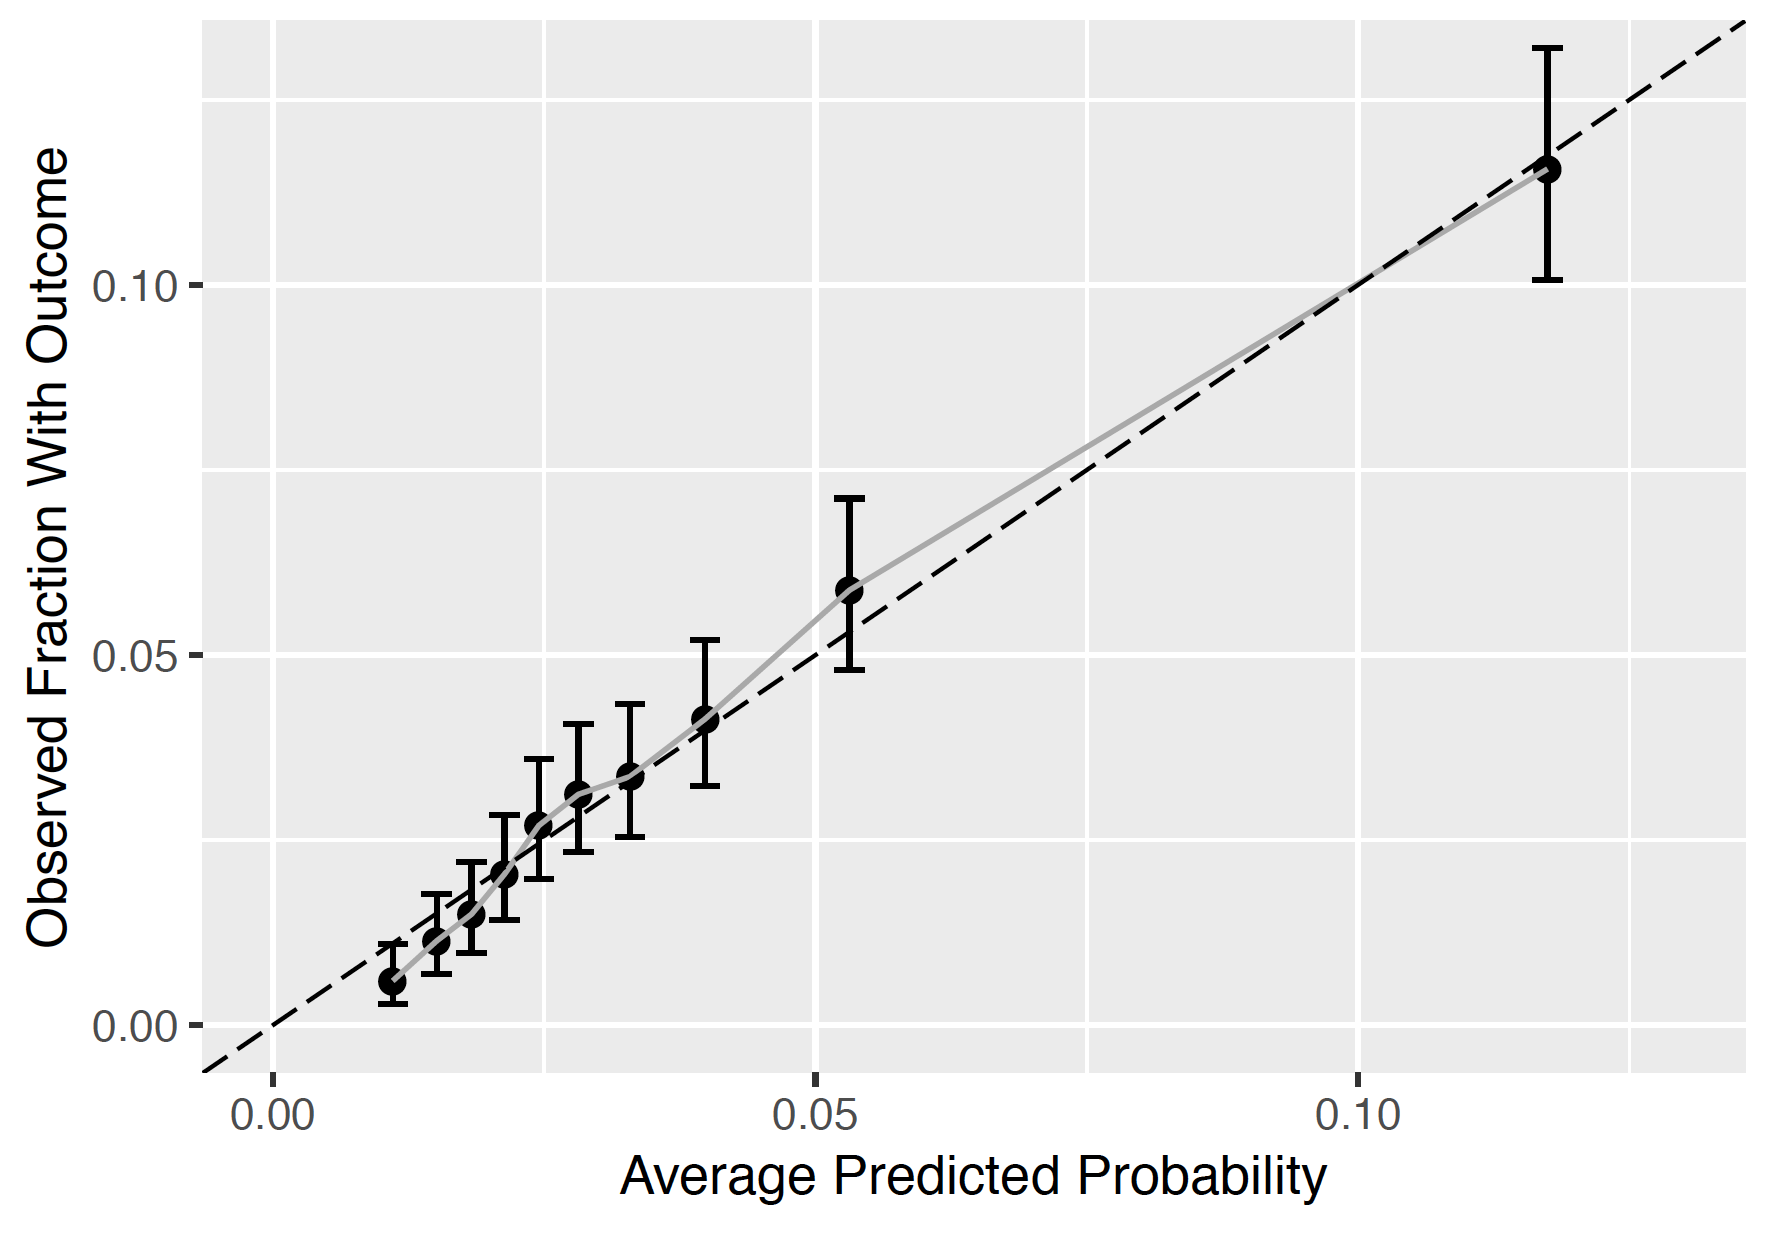
\includegraphics{sparseCalibration.png}
\caption{Calibration Plot}
\end{figure}

The calibration plot shows how close the predicted risk is to the
observed risk. The diagonal dashed line thus indicates a perfectly
calibrated model. The ten (or fewer) dots represent the mean predicted
values for each quantile plotted against the observed fraction of people
in that quantile who had the outcome (observed fraction). The straight
black line is the linear regression using these 10 plotted quantile mean
predicted vs observed fraction points. The two blue straight lines
represented the 95\% lower and upper confidence intervals of the slope
of the fitted line.

\newpage

\subsection{Smooth Calibration plot}\label{smooth-calibration-plot}

\begin{figure}
\centering
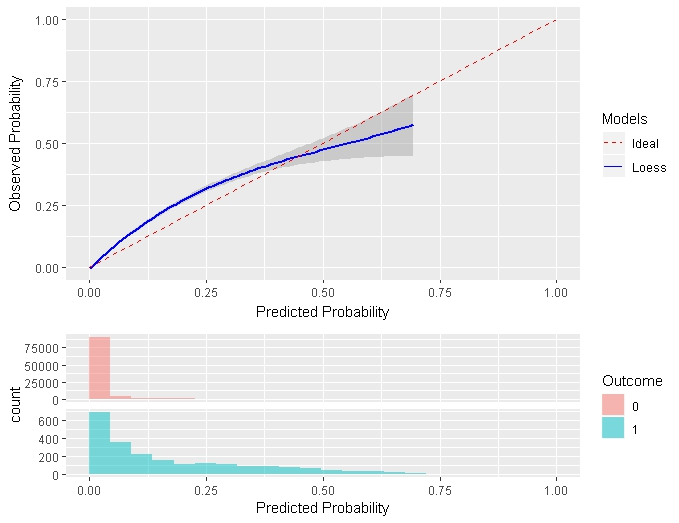
\includegraphics{smoothCalibration.jpeg}
\caption{Smooth Calibration plot}
\end{figure}

Similar to the traditional calibration shown above the Smooth
Calibration plot shows the relationship between predicted and observed
risk. the major difference is that the smooth fit allows for a more fine
grained examination of this. Whereas the traditional plot will be
heavily influenced by the areas with the highest density of data the
smooth plot will provide the same information for this region as well as
a more accurate interpretation of areas with lower density. the plot
also contains information on the distribution of the outcomes relative
to predicted risk.

However the increased information game comes at a computational cost. It
is recommended to use the traditional plot for examination and then to
produce the smooth plot for final versions.

\newpage

\subsection{Preference distribution
plots}\label{preference-distribution-plots}

\begin{figure}
\centering
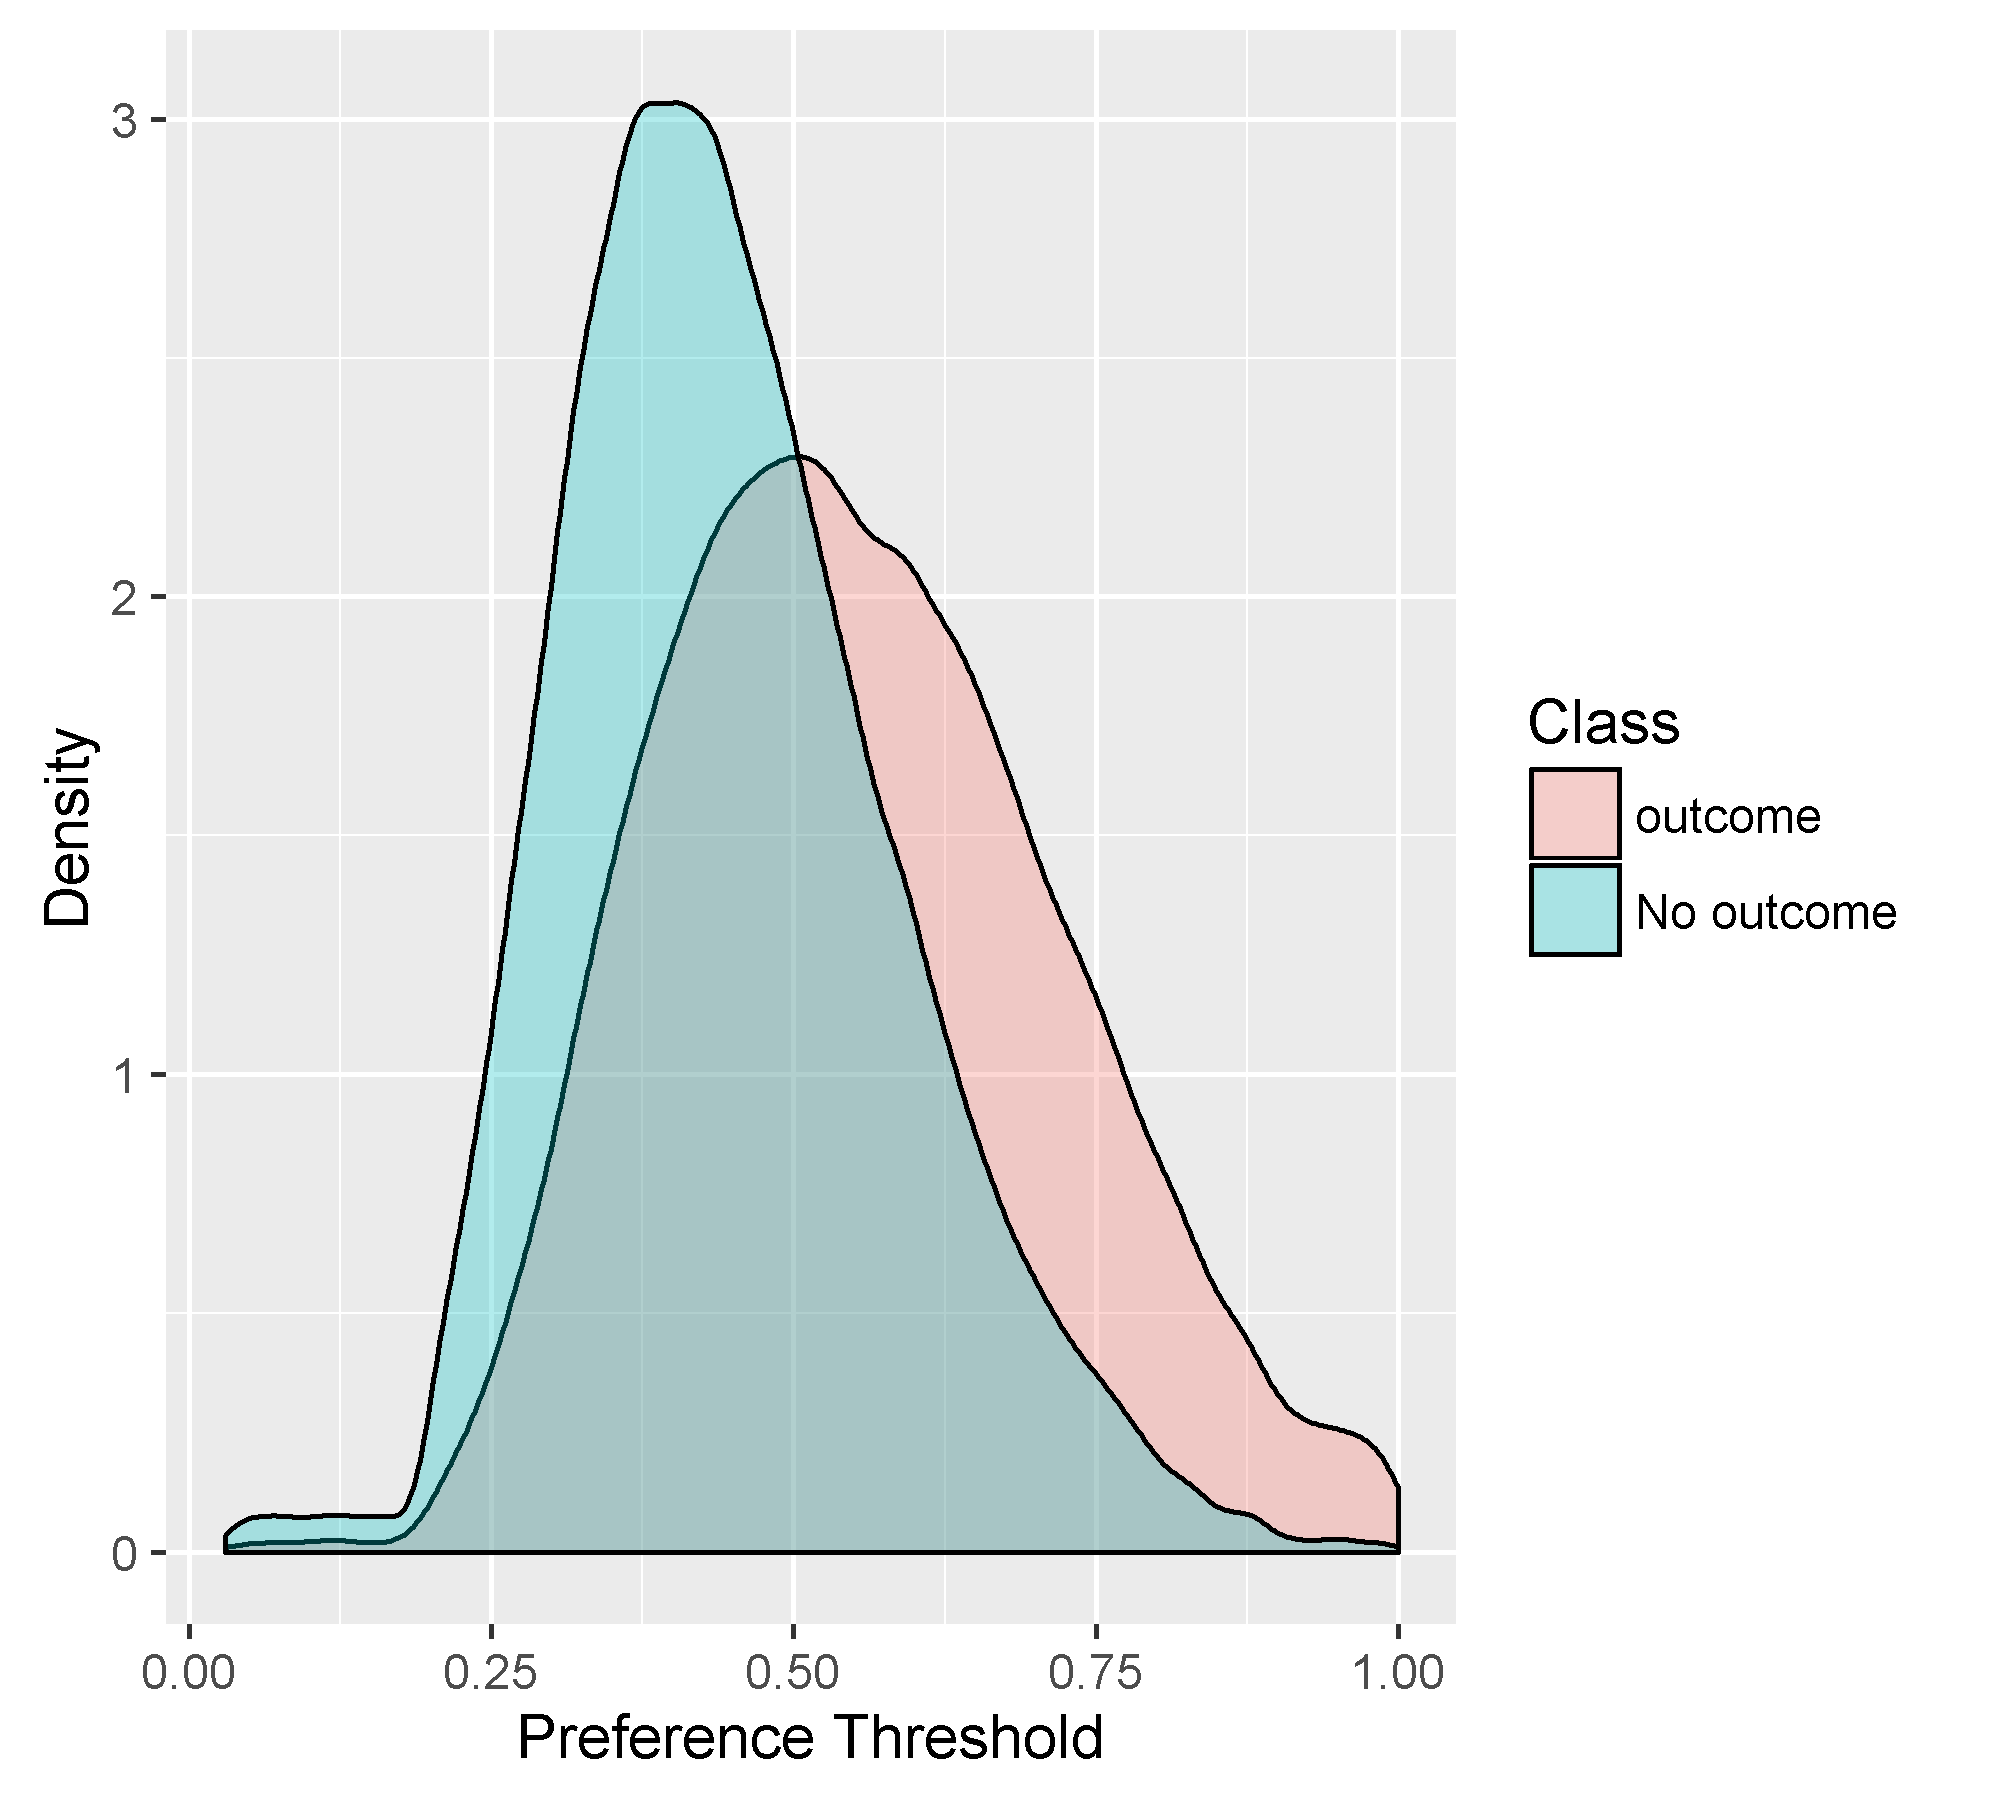
\includegraphics{preferencePDF.png}
\caption{Preference Plot}
\end{figure}

The preference distribution plots are the preference score distributions
corresponding to i) people in the test set with the outcome (red) and
ii) people in the test set without the outcome (blue).

\newpage

\subsection{Box plots}\label{box-plots}

\begin{figure}
\centering
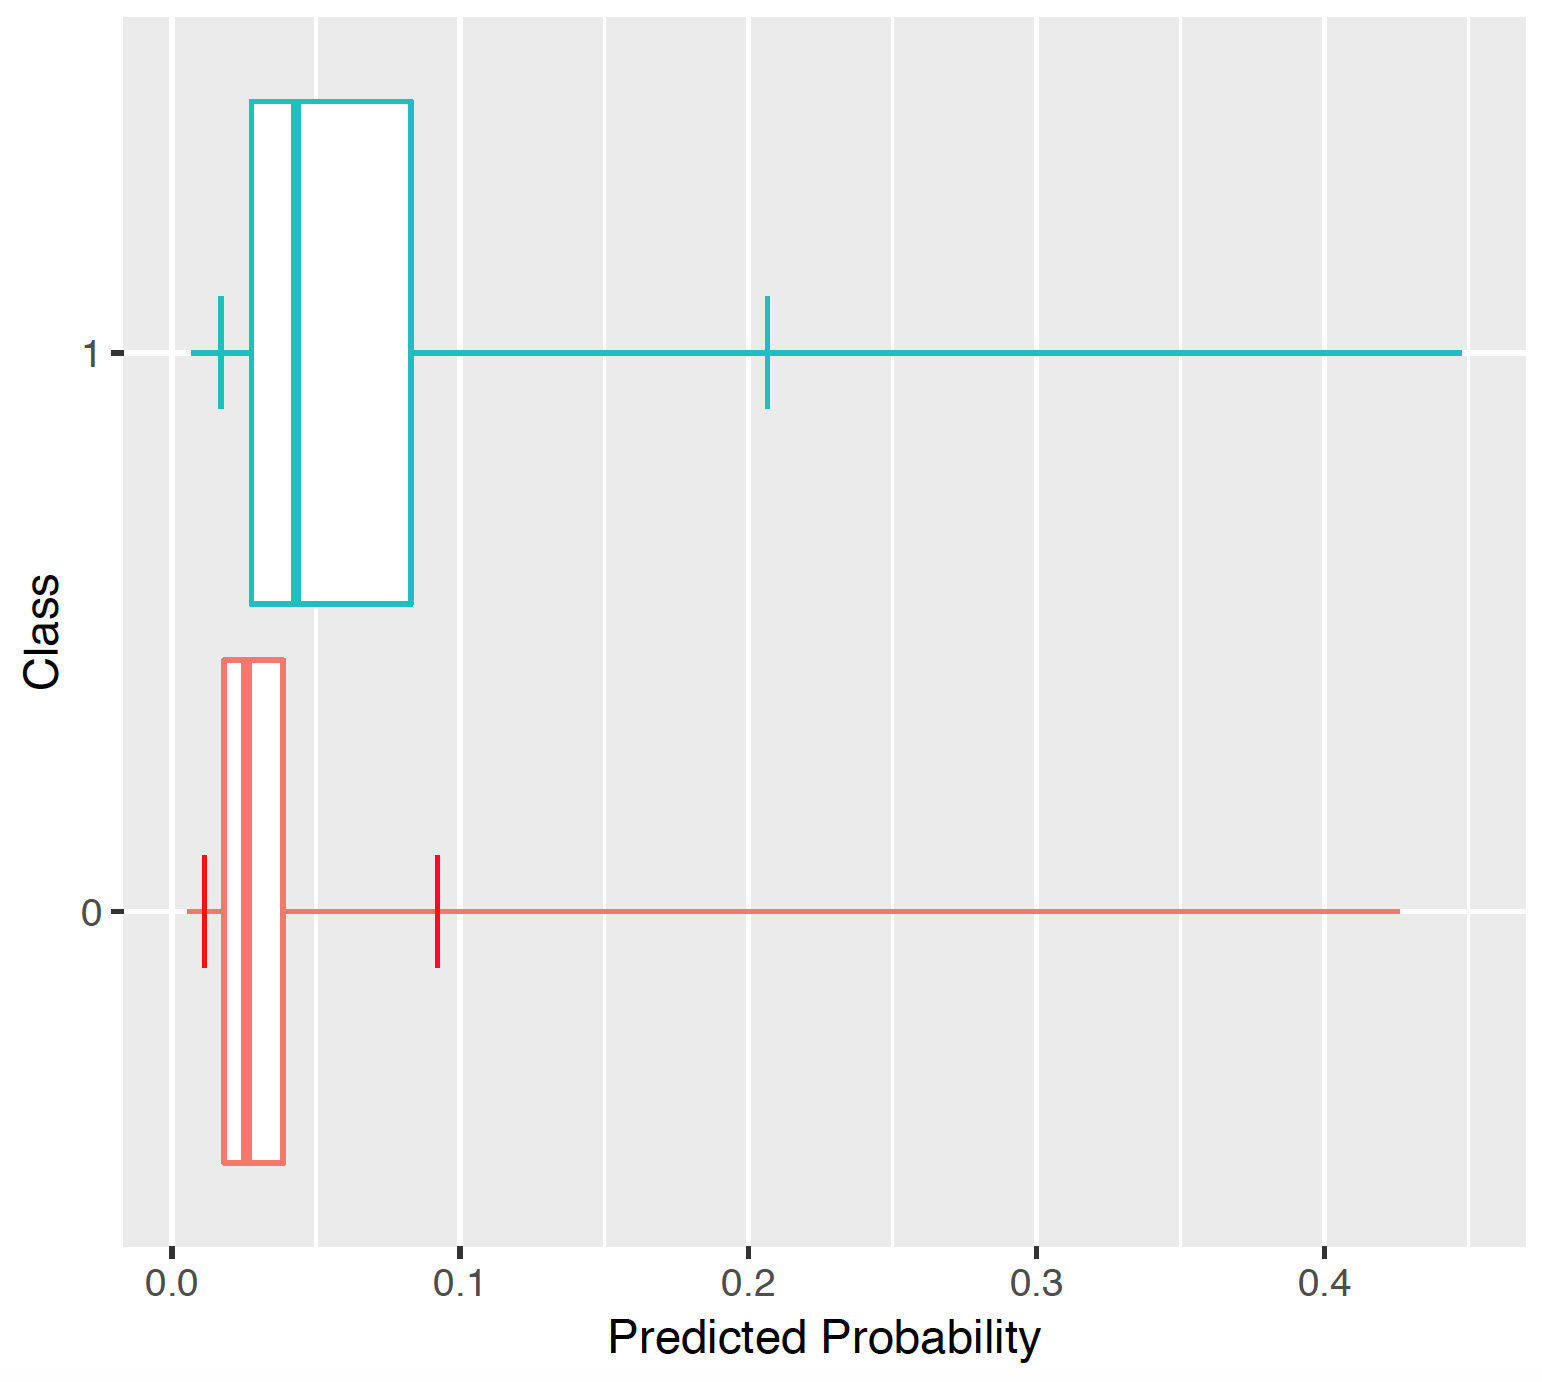
\includegraphics{predictionDistribution.png}
\caption{Prediction Distribution Box Plot}
\end{figure}

The prediction distribution boxplots are box plots for the predicted
risks of the people in the test set with the outcome (class 1: blue) and
without the outcome (class 0: red).

The box plots in the Figure above show that the predicted probability of
the outcome is indeed higher for those with the outcome but there is
also overlap between the two distribution which lead to an imperfect
discrimination.

\newpage

\subsection{Test-Train similarity
plot}\label{test-train-similarity-plot}

\begin{figure}
\centering
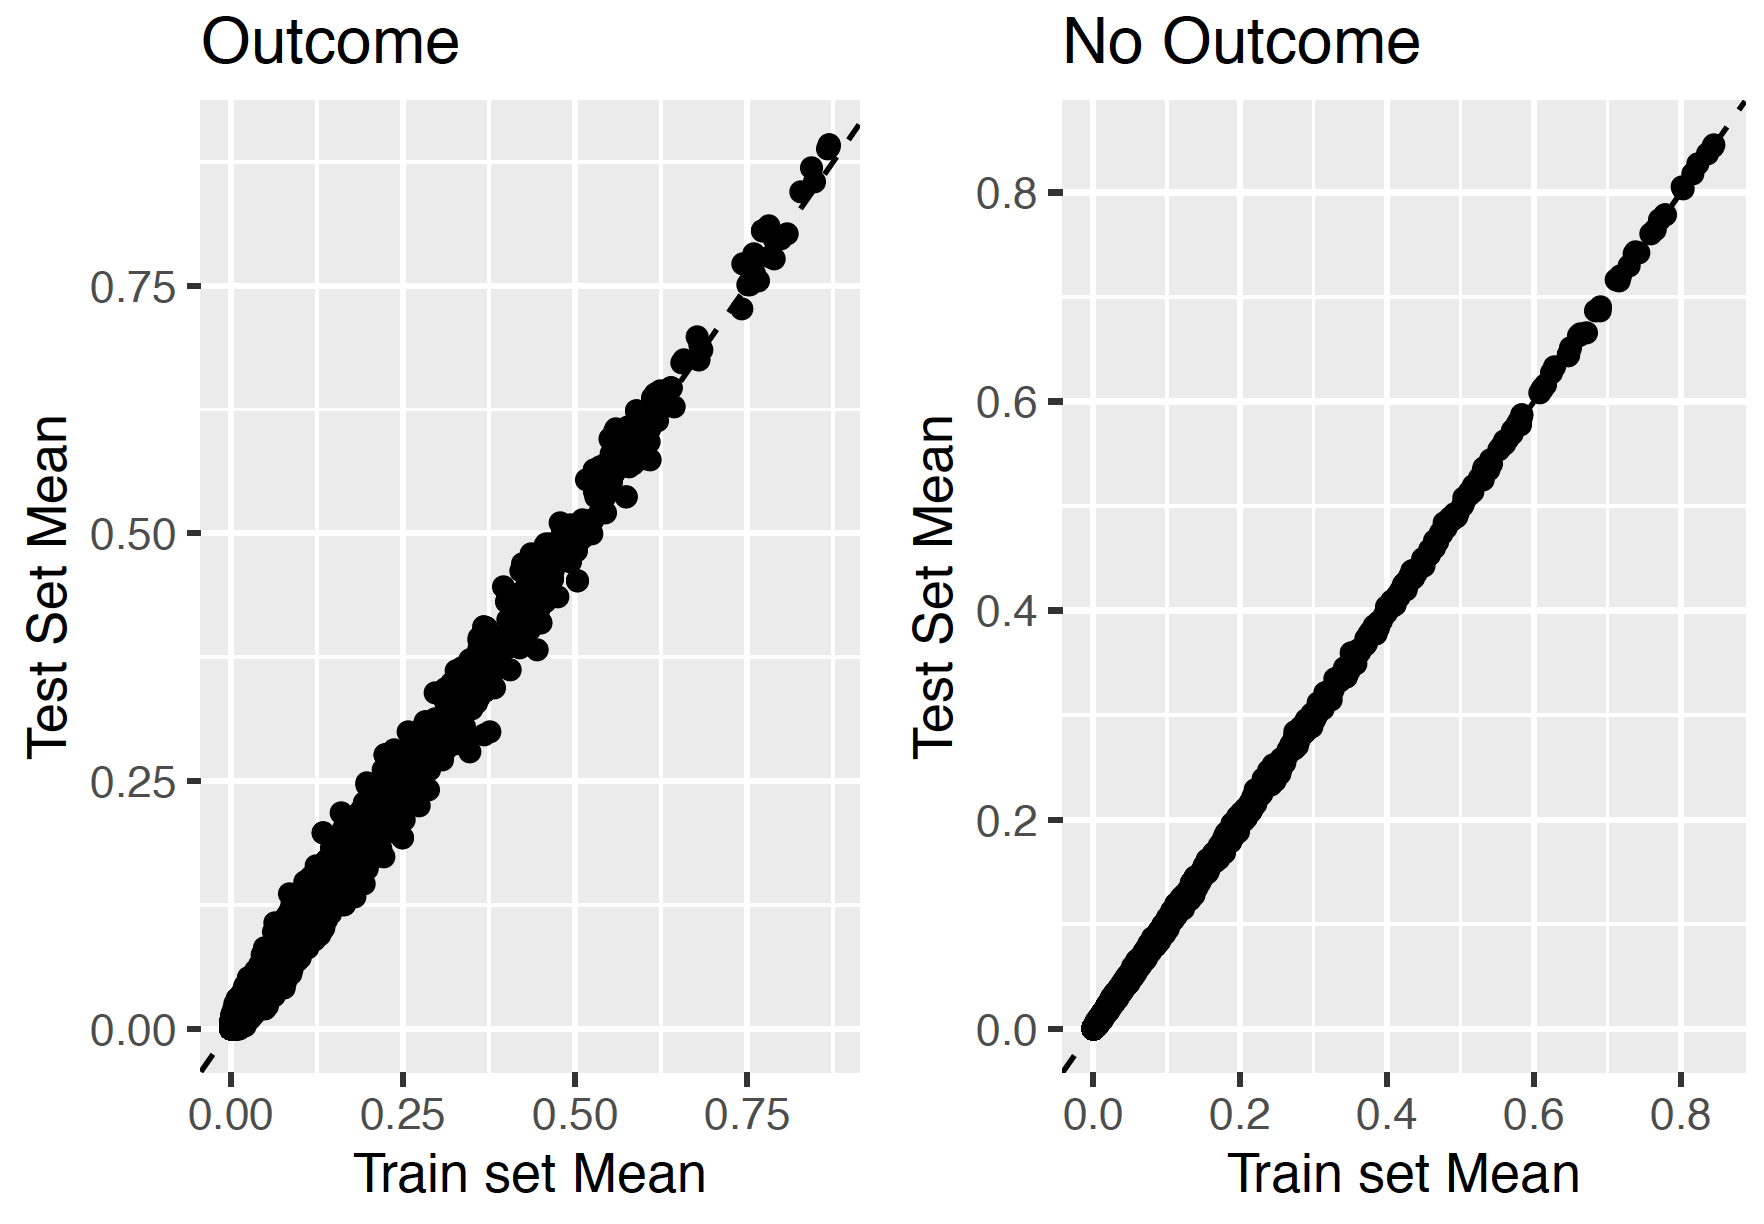
\includegraphics{generalizability.png}
\caption{Similarity plots of train and test set}
\end{figure}

The test-train similarity is presented by plotting the mean covariate
values in the train set against those in the test set for people with
and without the outcome.

The results for our example of re-hospitalization look very promising
since the mean values of the covariates are on the diagonal.

\newpage

\subsection{Variable scatter plot}\label{variable-scatter-plot}

The variable scatter plot shows the mean covariate value for the people
with the outcome against the mean covariate value for the people without
the outcome. The size and color of the dots correspond to the importance
of the covariates in the trained model (size of beta) and its direction
(sign of beta with green meaning positive and red meaning negative),
respectivily.

The plot shows that the mean of most of the covariates is higher for
subjects with the outcome compared to those without. Also there seem to
be a very predictive, but rare covariate with a high beta.

\begin{figure}
\centering
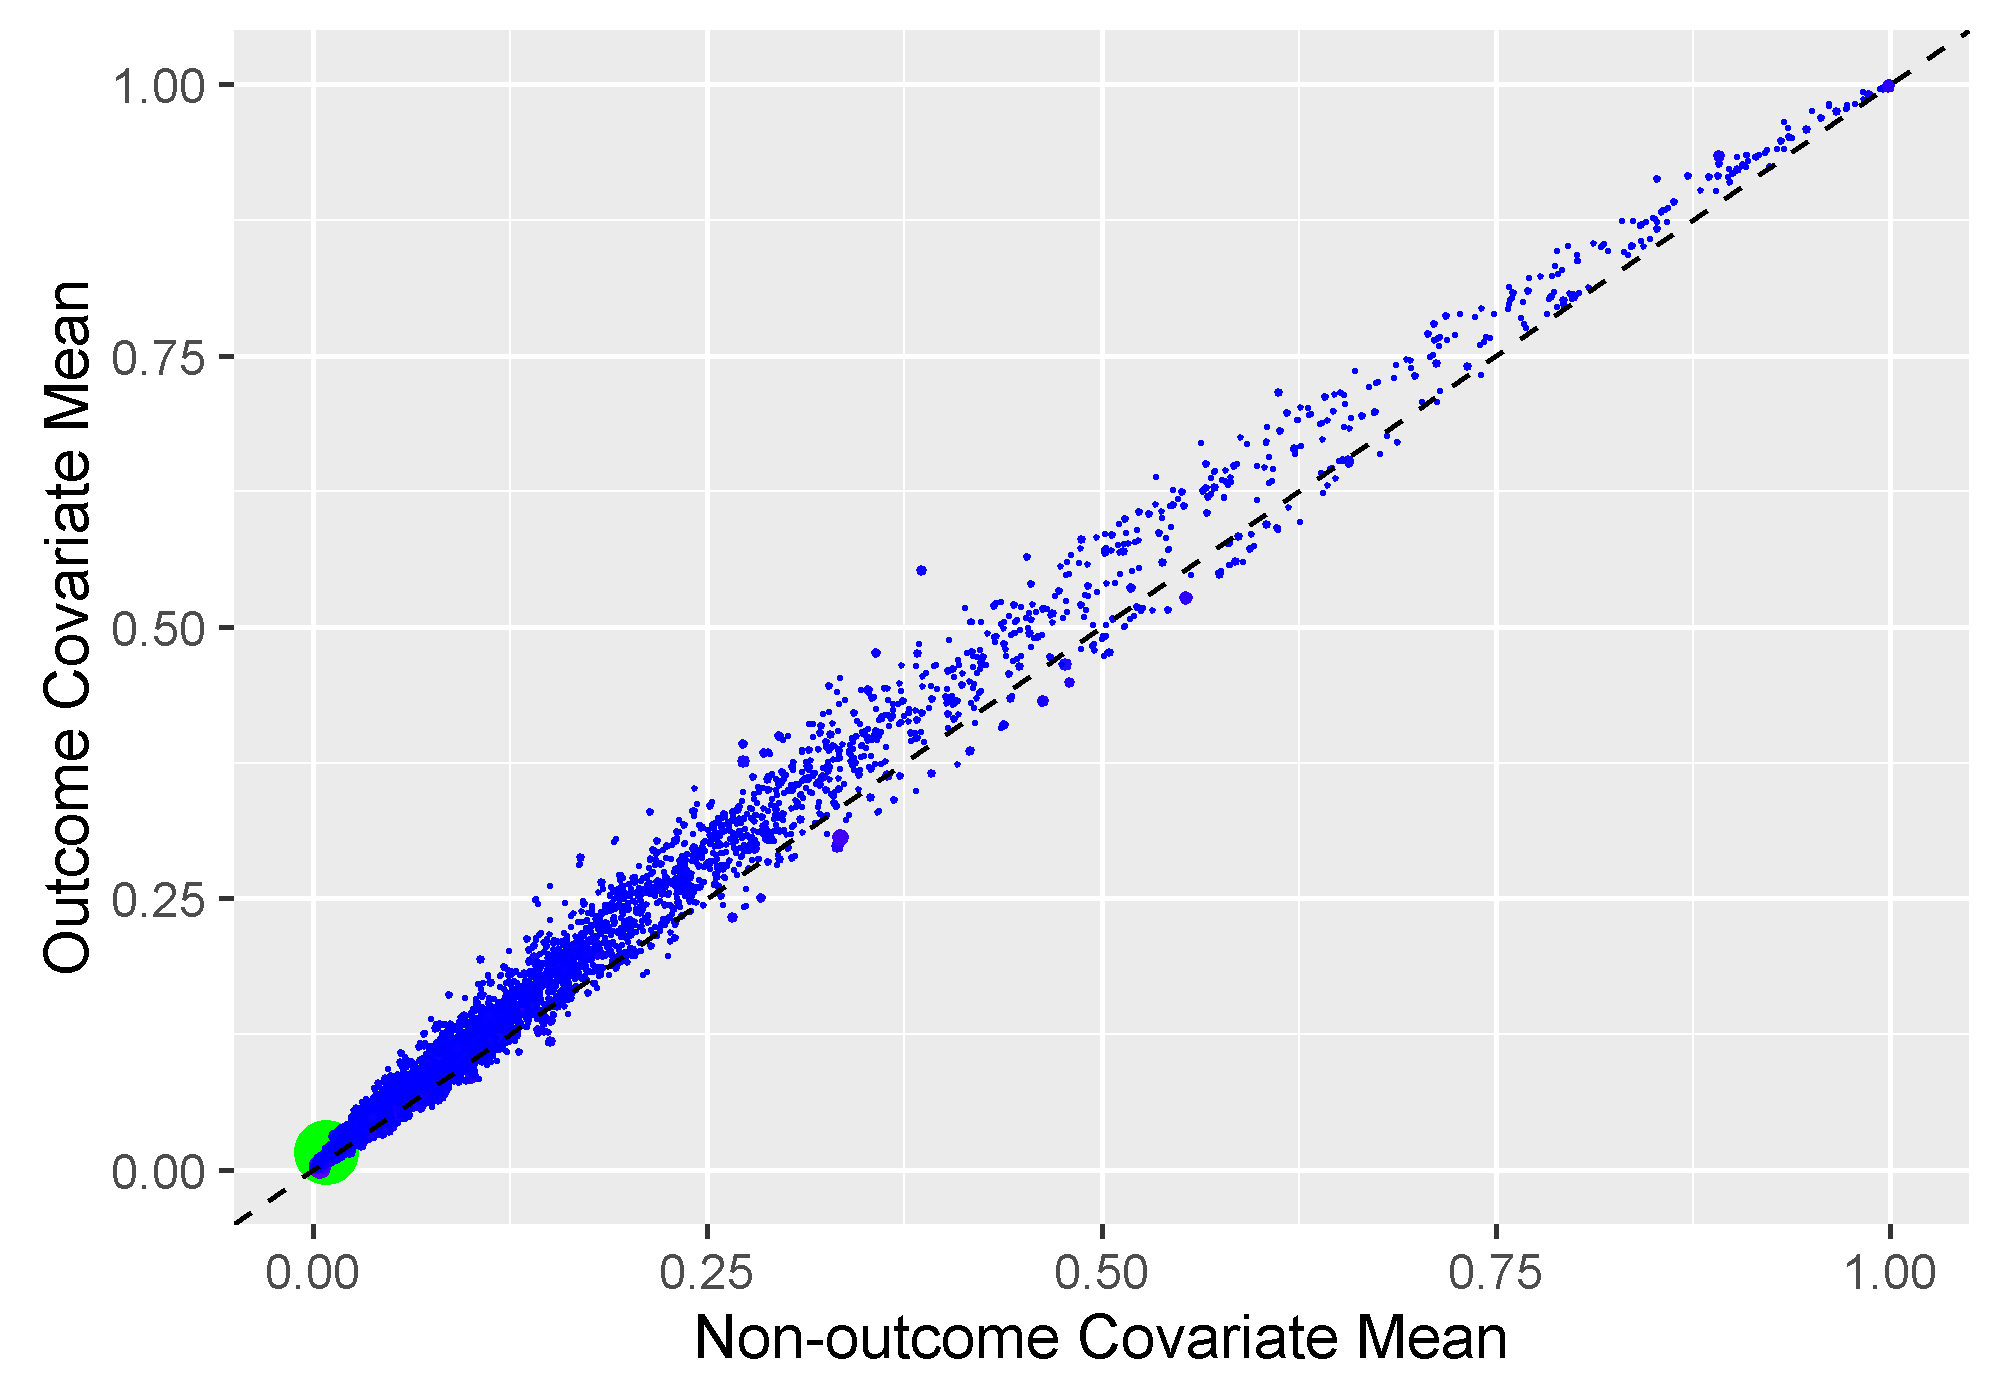
\includegraphics{variableScatterplot.png}
\caption{Variabel scatter Plot}
\end{figure}

\newpage

\subsection{Plot Precision Recall}\label{plot-precision-recall}

\begin{figure}
\centering
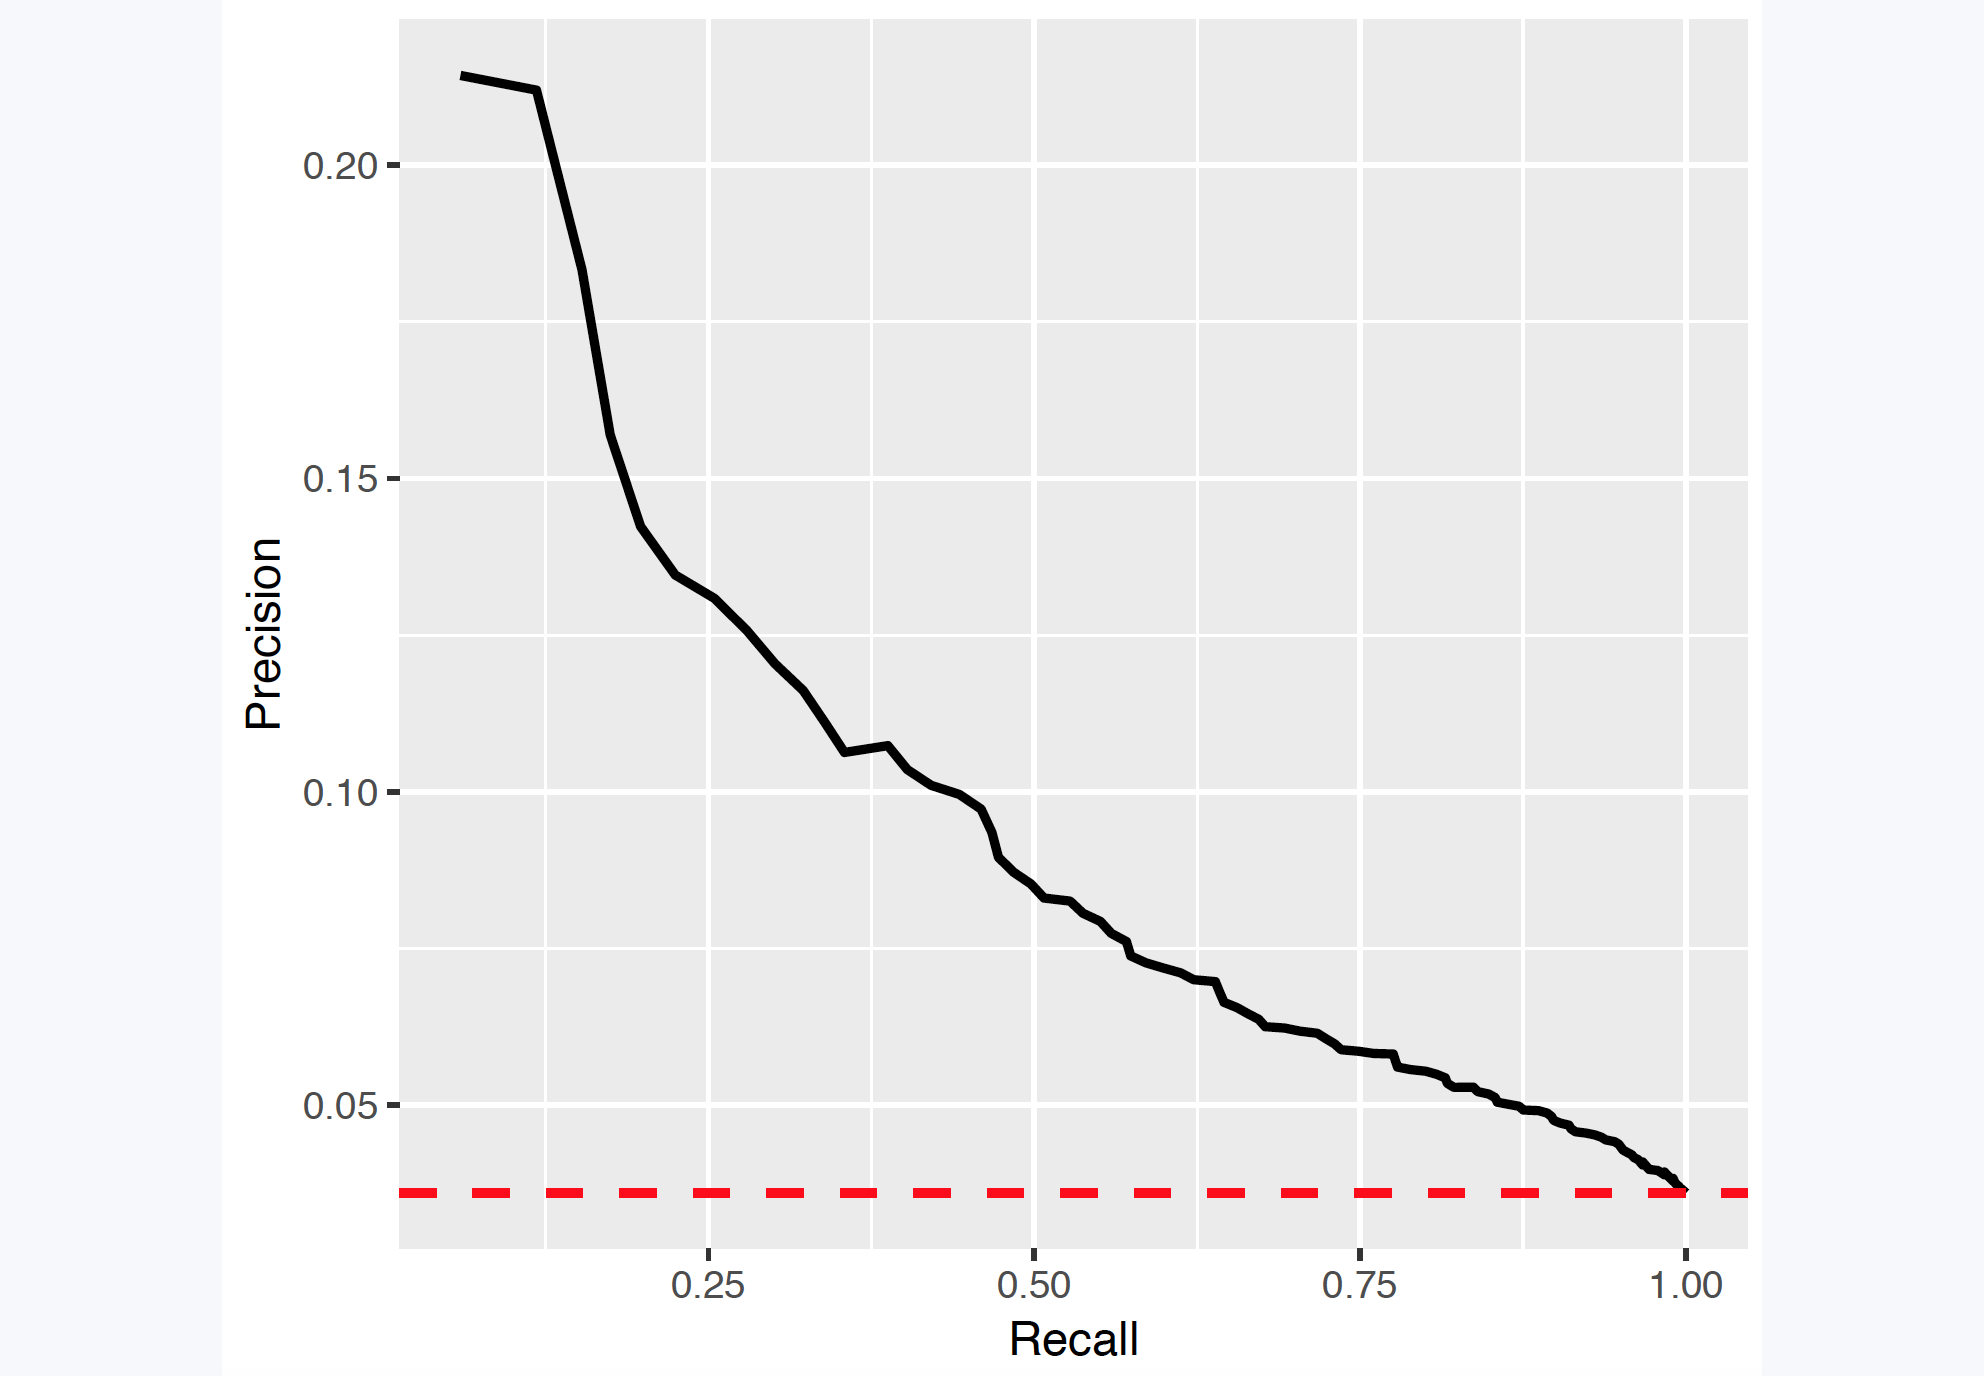
\includegraphics{precisionRecall.png}
\caption{Precision Recall Plot}
\end{figure}

Precision (P) is defined as the number of true positives (Tp) over the
number of true positives plus the number of false positives (Fp).

\begin{Shaded}
\begin{Highlighting}[]
\NormalTok{P <-}\StringTok{ }\NormalTok{Tp}\OperatorTok{/}\NormalTok{(Tp }\OperatorTok{+}\StringTok{ }\NormalTok{Fp)}
\end{Highlighting}
\end{Shaded}

Recall (R) is defined as the number of true positives (Tp) over the
number of true positives plus the number of false negatives (Fn).

\begin{Shaded}
\begin{Highlighting}[]
\NormalTok{R <-}\StringTok{ }\NormalTok{Tp}\OperatorTok{/}\NormalTok{(Tp }\OperatorTok{+}\StringTok{ }\NormalTok{Fn)}
\end{Highlighting}
\end{Shaded}

These quantities are also related to the (F1) score, which is defined as
the harmonic mean of precision and recall.

\begin{Shaded}
\begin{Highlighting}[]
\NormalTok{F1 <-}\StringTok{ }\DecValTok{2} \OperatorTok{*}\StringTok{ }\NormalTok{P }\OperatorTok{*}\StringTok{ }\NormalTok{R}\OperatorTok{/}\NormalTok{(P }\OperatorTok{+}\StringTok{ }\NormalTok{R)}
\end{Highlighting}
\end{Shaded}

Note that the precision can either decrease or increase if the threshold
is lowered. Lowering the threshold of a classifier may increase the
denominator, by increasing the number of results returned. If the
threshold was previously set too high, the new results may all be true
positives, which will increase precision. If the previous threshold was
about right or too low, further lowering the threshold will introduce
false positives, decreasing precision.

For Recall the demoninator does not depend on the classifier threshold
(Tp+Fn is a constant). This means that lowering the classifier threshold
may increase recall, by increasing the number of true positive results.
It is also possible that lowering the threshold may leave recall
unchanged, while the precision fluctuates.

\newpage

\subsection{Demographic Summary plot}\label{demographic-summary-plot}

\begin{figure}
\centering
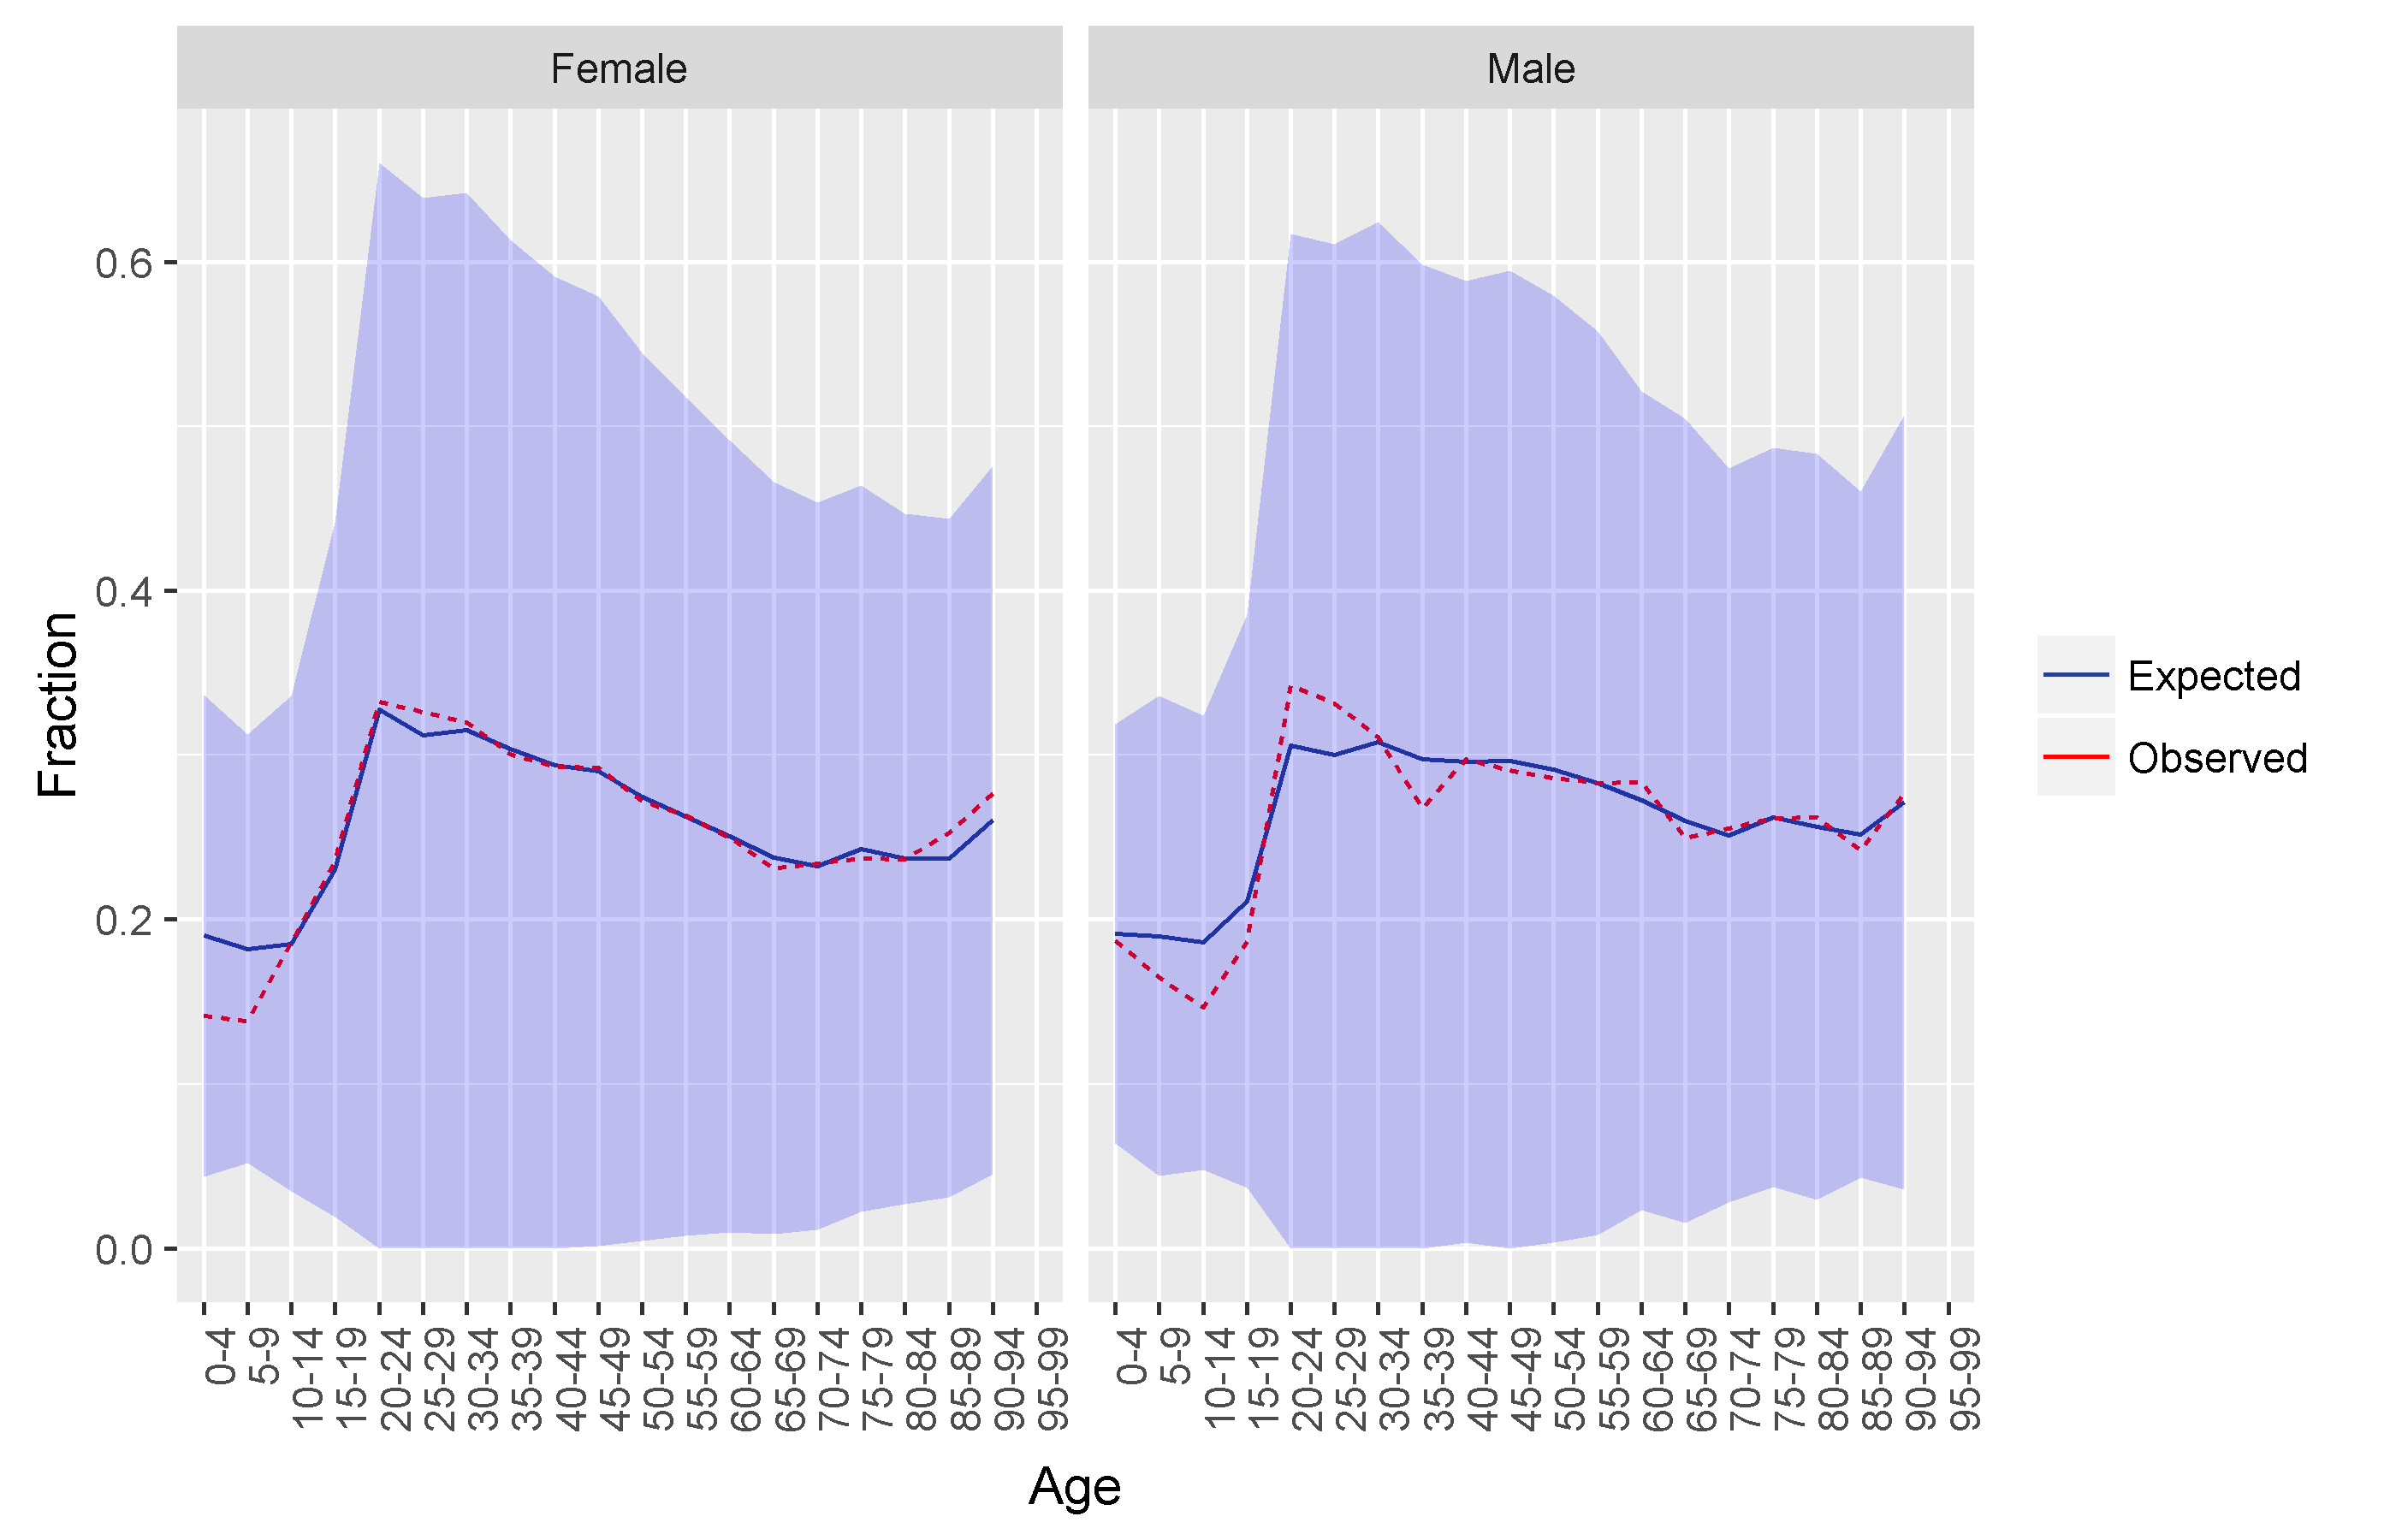
\includegraphics{demographicSummary.png}
\caption{Demographic Summary Plot}
\end{figure}

This plot shows for females and males the expected and observed risk in
different age groups together with a confidence area.

\newpage

\section{External validation}\label{external-validation}

We recommend to always perform external validation, i.e.~apply the final
model on as much new datasets as feasible and evaluate its performance.

\begin{Shaded}
\begin{Highlighting}[]
\CommentTok{# load the trained model}
\NormalTok{plpModel <-}\StringTok{ }\KeywordTok{loadPlpModel}\NormalTok{(}\KeywordTok{getwd}\NormalTok{(),}\StringTok{'model'}\NormalTok{)}

\CommentTok{#load the new plpData and create the population}
\NormalTok{plpData <-}\StringTok{ }\KeywordTok{loadPlpData}\NormalTok{(}\KeywordTok{getwd}\NormalTok{(),}\StringTok{'data'}\NormalTok{)}
\NormalTok{population <-}\StringTok{ }\KeywordTok{createStudyPopulation}\NormalTok{(plpData, }
\DataTypeTok{outcomeId =} \DecValTok{2}\NormalTok{, }
\DataTypeTok{includeAllOutcomes =} \OtherTok{TRUE}\NormalTok{, }
\DataTypeTok{firstExposureOnly =} \OtherTok{TRUE}\NormalTok{, }
\DataTypeTok{washoutPeriod =} \DecValTok{365}\NormalTok{, }
\DataTypeTok{removeSubjectsWithPriorOutcome =} \OtherTok{TRUE}\NormalTok{, }
\DataTypeTok{priorOutcomeLookback =} \DecValTok{365}\NormalTok{,}
\DataTypeTok{riskWindowStart =} \DecValTok{1}\NormalTok{,}
\DataTypeTok{requireTimeAtRisk =} \OtherTok{FALSE}\NormalTok{,}
\DataTypeTok{riskWindowEnd =} \DecValTok{365}
\NormalTok{)}

\CommentTok{# apply the trained model on the new data}
\NormalTok{validationResults <-}\StringTok{ }\KeywordTok{applyModel}\NormalTok{(population,plpData,plpModel)}
\end{Highlighting}
\end{Shaded}

To make things easier we also provide a function for performing external
validation of a model across one or multiple datasets:

\begin{Shaded}
\begin{Highlighting}[]
\CommentTok{# load the trained model}
\NormalTok{plpResult <-}\StringTok{ }\KeywordTok{loadPlpResult}\NormalTok{(}\KeywordTok{getwd}\NormalTok{(),}\StringTok{'plpResult'}\NormalTok{)}

\NormalTok{connectionDetails <-}\StringTok{ }\KeywordTok{createConnectionDetails}\NormalTok{(}\DataTypeTok{dbms =} \StringTok{"postgresql"}\NormalTok{, }
                                             \DataTypeTok{server =} \StringTok{"localhost/ohdsi"}\NormalTok{, }
                                             \DataTypeTok{user =} \StringTok{"joe"}\NormalTok{, }
                                             \DataTypeTok{password =} \StringTok{"supersecret"}\NormalTok{)}

\NormalTok{validation <-}\StringTok{ }\KeywordTok{externalValidatePlp}\NormalTok{(}\DataTypeTok{plpResult =}\NormalTok{ plpResult, }
                                  \DataTypeTok{connectionDetails =}\NormalTok{ connectionDetails,}
                                  \DataTypeTok{validationSchemaTarget =} \StringTok{'new_cohort_schema'}\NormalTok{,}
                                  \DataTypeTok{validationSchemaOutcome =} \StringTok{'new_cohort_schema'}\NormalTok{,}
                                  \DataTypeTok{validationSchemaCdm =} \StringTok{'new_cdm_schema'}\NormalTok{, }
                                  \DataTypeTok{validationTableTarget =} \StringTok{'cohort_table'}\NormalTok{,}
                                  \DataTypeTok{validationTableOutcome =} \StringTok{'cohort_table'}\NormalTok{, }
                                  \DataTypeTok{validationIdTarget =} \StringTok{'cohort_id'}\NormalTok{, }
                                  \DataTypeTok{validationIdOutcome =} \StringTok{'outcome_id'}\NormalTok{, }
                                  \DataTypeTok{keepPrediction =}\NormalTok{ T}
\NormalTok{                                  )}
\end{Highlighting}
\end{Shaded}

This will extract the new plpData from the specified schemas and cohort
tables. It will then apply the same population settings and the trained
plp model. Finally, it will evaluate the performance and return the
standard output as \texttt{validation\$performance} and if
keepPrediction is TRUE then it will also return the prediction on the
population as \texttt{validation\$prediction}. They can be inserted into
the shiny app for viewing the model and validation by running:
\texttt{viewPlp(runPlp=plpResult,\ validatePlp=validation\ )}.

If you want to validate on multiple databases available you can insert
the new schemas and cohort tables as a list:

\begin{Shaded}
\begin{Highlighting}[]
\CommentTok{# load the trained model}
\NormalTok{plpResult <-}\StringTok{ }\KeywordTok{loadPlpResult}\NormalTok{(}\KeywordTok{getwd}\NormalTok{(),}\StringTok{'plpResult'}\NormalTok{)}

\NormalTok{connectionDetails <-}\StringTok{ }\KeywordTok{createConnectionDetails}\NormalTok{(}\DataTypeTok{dbms =} \StringTok{"postgresql"}\NormalTok{, }
                                             \DataTypeTok{server =} \StringTok{"localhost/ohdsi"}\NormalTok{, }
                                             \DataTypeTok{user =} \StringTok{"joe"}\NormalTok{, }
                                             \DataTypeTok{password =} \StringTok{"supersecret"}\NormalTok{)}

\NormalTok{validation <-}\StringTok{ }\KeywordTok{externalValidatePlp}\NormalTok{(}\DataTypeTok{plpResult =}\NormalTok{ plpResult, }
                                  \DataTypeTok{connectionDetails =}\NormalTok{ connectionDetails,}
                                  \DataTypeTok{validationSchemaTarget =} \KeywordTok{list}\NormalTok{(}\StringTok{'new_cohort_schema1'}\NormalTok{,}
                                                                \StringTok{'new_cohort_schema2'}\NormalTok{),}
                                  \DataTypeTok{validationSchemaOutcome =} \KeywordTok{list}\NormalTok{(}\StringTok{'new_cohort_schema1'}\NormalTok{,}
                                                                 \StringTok{'new_cohort_schema2'}\NormalTok{),}
                                  \DataTypeTok{validationSchemaCdm =} \KeywordTok{list}\NormalTok{(}\StringTok{'new_cdm_schema1'}\NormalTok{,}
                                                             \StringTok{'new_cdm_schema2'}\NormalTok{), }
                                  \DataTypeTok{validationTableTarget =} \KeywordTok{list}\NormalTok{(}\StringTok{'new_cohort_table1'}\NormalTok{,}
                                                               \StringTok{'new_cohort_table2'}\NormalTok{),}
                                  \DataTypeTok{validationTableOutcome =} \KeywordTok{list}\NormalTok{(}\StringTok{'new_cohort_table1'}\NormalTok{,}
                                                                \StringTok{'new_cohort_table2'}\NormalTok{),}
                                  \DataTypeTok{validationIdTarget =} \StringTok{'cohort_id'}\NormalTok{, }
                                  \DataTypeTok{validationIdOutcome =} \StringTok{'outcome_id'}\NormalTok{, }
                                  \DataTypeTok{keepPrediction =}\NormalTok{ T}
\NormalTok{                                  )}
\end{Highlighting}
\end{Shaded}

\section{Demos}\label{demos}

We have added several demos in the package that run on simulated data:

\begin{Shaded}
\begin{Highlighting}[]
\CommentTok{# Show all demos in our package: }
 \KeywordTok{demo}\NormalTok{(}\DataTypeTok{package =} \StringTok{"PatientLevelPrediction"}\NormalTok{)}

\CommentTok{# To run the SingleModelDemo for example use this call}
 \KeywordTok{demo}\NormalTok{(}\StringTok{"SingleModelDemo"}\NormalTok{, }\DataTypeTok{package =} \StringTok{"PatientLevelPrediction"}\NormalTok{)}
\end{Highlighting}
\end{Shaded}

\newpage

\section{Acknowledgments}\label{acknowledgments}

Considerable work has been dedicated to provide the
\texttt{PatientLevelPrediction} package.

\begin{Shaded}
\begin{Highlighting}[]
\KeywordTok{citation}\NormalTok{(}\StringTok{"PatientLevelPrediction"}\NormalTok{)}
\end{Highlighting}
\end{Shaded}

\begin{verbatim}
## 
##   Jenna Reps, Martijn J. Schuemie, Marc A. Suchard, Patrick B.
##   Ryan and Peter R. Rijnbeek (2018). PatientLevelPrediction:
##   Package for patient level prediction using data in the OMOP
##   Common Data Model. R package version 2.0.5.
## 
## A BibTeX entry for LaTeX users is
## 
##   @Manual{,
##     title = {PatientLevelPrediction: Package for patient level prediction using data in the OMOP Common Data
## Model},
##     author = {Jenna Reps and Martijn J. Schuemie and Marc A. Suchard and Patrick B. Ryan and Peter R. Rijnbeek},
##     year = {2018},
##     note = {R package version 2.0.5},
##   }
\end{verbatim}

Further, \texttt{PatientLevelPrediction} makes extensive use of the
\texttt{Cyclops} package.

\begin{Shaded}
\begin{Highlighting}[]
\KeywordTok{citation}\NormalTok{(}\StringTok{"Cyclops"}\NormalTok{)}
\end{Highlighting}
\end{Shaded}

\begin{verbatim}
## 
## To cite Cyclops in publications use:
## 
## Suchard MA, Simpson SE, Zorych I, Ryan P, Madigan D (2013).
## "Massive parallelization of serial inference algorithms for
## complex generalized linear models." _ACM Transactions on Modeling
## and Computer Simulation_, *23*, 10. <URL:
## http://dl.acm.org/citation.cfm?id=2414791>.
## 
## A BibTeX entry for LaTeX users is
## 
##   @Article{,
##     author = {M. A. Suchard and S. E. Simpson and I. Zorych and P. Ryan and D. Madigan},
##     title = {Massive parallelization of serial inference algorithms for complex generalized linear models},
##     journal = {ACM Transactions on Modeling and Computer Simulation},
##     volume = {23},
##     pages = {10},
##     year = {2013},
##     url = {http://dl.acm.org/citation.cfm?id=2414791},
##   }
\end{verbatim}

\textbf{Please reference this paper if you use the PLP Package in your
work:}

\href{http://dx.doi.org/10.1093/jamia/ocy032}{Reps JM, Schuemie MJ,
Suchard MA, Ryan PB, Rijnbeek PR. Design and implementation of a
standardized framework to generate and evaluate patient-level prediction
models using observational healthcare data. J Am Med Inform Assoc.
2018;25(8):969-975.}

This work is supported in part through the National Science Foundation
grant IIS 1251151.


\end{document}
